\documentclass[12pt,draftcls,peerreview,onecolumn]{IEEEtran}
%\documentclass[10pt,conference,twocolumn]{IEEEtran}
%\documentclass[10pt,conference]{IEEEtran}
\usepackage{epsf}
\usepackage{amsmath,amssymb}
\usepackage{graphicx}
\usepackage{color}
\usepackage{cite}
\usepackage{multirow,tabularx}
\usepackage{ifthen}
% Add these after the document class declaration
\usepackage{times}
\usepackage{stackrel}
%\usepackage{hyperref}

\graphicspath{{./plots/}}
%\input{epsf.sty}
%\pagestyle{bfheadings}
%-------------------------------

%\input{commands.tex}

\renewcommand{\baselinestretch}{1.65}
\newcommand{\showfigure}{\boolean{true}}
%\newcommand{\showfigure}{\boolean{false}}

\newcommand{\hide}[1]{\ifthenelse{\boolean{false}}{#1}{}}

%\include{../../commonHeader}
%%%%%%%%%%%%%%%%%%%%%%
% Theorems, etc.

\newtheorem{theorem}{{\bf Theorem}}
\newtheorem{lemma}{{\bf Lemma}}
\newtheorem{proposition}[theorem]{Proposition}
\newtheorem{corollary}{{\bf Corollary}}

%\newenvironment{proof}[1][Proof]{\begin{trivlist}
%\item[\hskip \labelsep {\bfseries #1}]}{\end{trivlist}}

%\newtheorem{defn}{Definition}
\newenvironment{definition}[1][Definition]{\begin{trivlist}
\item[\hskip \labelsep {\bfseries #1}]}{\end{trivlist}}

\newenvironment{example}[1][Example]{\begin{trivlist}
\item[\hskip \labelsep {\bfseries #1}]}{\end{trivlist}}

\newenvironment{remark}[1][Remark]{\begin{trivlist}
\item[\hskip \labelsep {\bfseries #1}]}{\end{trivlist}}

\newcommand{\qed}{\nobreak \ifvmode \relax \else
      \ifdim\lastskip<1.5em \hskip-\lastskip
      \hskip1.5em plus0em minus0.5em \fi \nobreak
      \vrule height0.75em width0.5em depth0.25em\fi}


\newtheorem{fact}{Fact}
\newtheorem{obs}{Observation}

%%%%%%%%%%%%%%%%%%%%%%
% Environments

\newcommand{\barr}{\begin{array}}
\newcommand{\earr}{\end{array}}



%%%%%%%%%%%%%%%%%%%%%%
% References

\newcommand{\eqn}[1]{(\ref{#1})}

%%%%%%%%%%%%%%%%%%%%%%
% Brackets

\newcommand{\brac}[1]{\left({#1}\right)}
\newcommand{\sbrac}[1]{\left[{#1}\right]}
\newcommand{\cbrac}[1]{\left\{{#1}\right\}}

\newcommand{\floor}[1]{\left\lfloor{#1}\right\rfloor}

%%%%%%%%%%%%%%%%%%%%%%
% Misc

\newcommand{\expc}[2][]{E_{#1}\left[{#2}\right]}

\newcommand{\set}[1]{\{#1\}}

\newcommand{\ul}{\underline}
\newcommand{\smq}[1]{{\it #1}}
\newcommand{\ave}[1]{\overline{#1}}

\newcommand{\recip}[1]{\frac{1}{{#1}}}

%%%%%%%%%%%%%%%%%%%%%%
% Indicator function

\newcommand{\indic}[1]{I_{\cbrac{#1}}}

%%%%%%%%%%%%%%%%%%%%%%
% Superscripts
\newcommand{\supth}{^{{\mathrm{th}}}}
\newcommand{\mth}{^{{\mathrm{th}}}}
\newcommand{\supnd}{^{{\mathrm{nd}}}}
\newcommand{\suprd}{^{{\mathrm{rd}}}}


%%%%%%%%%%%%%%%%%%%%%%
% Combinatorics

\newcommand{\nchoosek}[2]{\left(\begin{array}{c}
                                {#1} \\ {#2}
                             \end{array}
                        \right)}

%%%%%%%%%%%%%%%%%%%%%%
% Symbols
\newcommand{\CN}{{\cal CN}}
\newcommand{\db}{{\mathrm dB}}
\newcommand{\Om}{\widehat{\Omega}}

\newcommand{\define}{\triangleq}
%\newcommand{\define}{\stackrel{\triangle}{=}}
%\newcommand{\implies}{\Rightarrow}
%\newcommand{\tendsto}{\rightarrow}
\newcommand{\tendsto}{\to}

\newcommand{\degree}{^{\circ}}
\newcommand{\kroneck}{\otimes}

%%%%%%%%%%%%%%%%%%%%%%
% Special phrases

\newcommand{\ie}{{i.e.}}
\newcommand{\eg}{{e.g.}}
\newcommand{\etal}{{et al.}}
\newcommand{\wrt}{w.r.t.}
\newcommand{\vs}{{vs.}}

%%%%%%%%%%%%%%%%%%%%%%
% Matrix related

\newcommand{\tvec}{\text{vec}} % \vec is already defined
\newcommand{\mtx}[1]{{\bf #1}} % matrix
\newcommand{\mtxg}[1]{{\boldsymbol #1}} % matrix for greek symbol

\newcommand{\trp}{\text{T}} % transpose
\newcommand{\trc}[1]{\text{Tr}\left\{{#1}\right\}} % trace

%%%%%%%%%%%%%%%%%%%%%%
% Special matrices


\newcommand{\mzero}{\mtx{0}}

%%%%%%%%%%%%%%%%%%%%%%
% Principal sub-matrix

\newcommand{\princ}[2]{{#2}^{({#1})}}
\newcommand{\princsup}[3]{{{#2}^{({#1})^{#3}}}}

%%%%%%%%%%%%%%%%%%%%%%
% Probability related

\newcommand{\EX}{\bf{E}} % expectation operator
\newcommand{\expect}[1]{{\bf{E}}\left[{#1}\right]}
\newcommand{\expectpow}[2]{{\bf{E}}^{#2}\left[{#1}\right]}
\newcommand{\explow}[2]{{\bf{E}}_{#1}\left[{#2}\right]}
\newcommand{\prob}[1]{\text{Pr}\brac{#1}}
\newcommand{\pr}{{\text{Pr}}}

%%%%%%%%%%%%%%%%%%%%%%
% Derivatives

\newcommand{\deriv}[2]{\frac{d{#1}}{d{#2}}}
\newcommand{\pderiv}[2]{\frac{\partial{#1}}{\partial{#2}}}

%%%%%%%%%%%%%%%%%%%%%%
% Slides

\newcommand{\bsp}{\begin{slide*}}
\newcommand{\esp}{\end{slide*}}
\newcommand{\bsl}{\begin{slide}}
\newcommand{\esl}{\end{slide}}
\newcommand{\vsp}[1]{\vspace{#1}}





%-------------------------------
% This paper's specific shortcuts

\newcommand{\nbm}[1]{{[\bf nbm: #1]}}
\newcommand{\vinod}[1]{[\textsl{v: #1}]}
\newcommand{\var}[1]{{\bf var}\left[{#1}\right]}
\newcommand{\opt}{\text{opt}}
\newcommand{\sth}{\text{th}}

\DeclareMathOperator*{\argmin}{arg\,min}
\DeclareMathOperator*{\argmax}{arg\,max}
%\newcommand{\var}{var}

\newcommand{\dv}{D}
\newcommand{\newdv}{{\cal D}^{\prime}}

\newcommand{\abs}[1]{\left\lvert{#1}\right\lvert}

%\newcommand{\err}{\text{Err}}

\newcommand{\given}{\arrowvert}
\newcommand{\givens}{\big\arrowvert}
\newcommand{\Given}{\Big\arrowvert}

\newcommand{\bMQAM}{b_{\text{QAM}}}
\newcommand{\bMPSK}{b_{\text{PSK}}}

\newcommand{\cMPSK}{c_{\text{PSK}}}
\newcommand{\cMQAM}{c_{\text{QAM}}}

%\newcommand{\opt}{\text{opt}}
%\newcommand{\asym}{\text{asm}}


%\newcommand{\err}{\text{Err}}


%% \newcommand{\alphaoptasm}{\alpha_{\opt}^{\asym}}
%% \newcommand{\betaoptasm}{\beta_{\opt}^{\asym}}


%\newcommand{\sepMPSK}{P_{\text{MPSK}}}

\newcommand{\limgamma}{\lim_{\gamma \tendsto \infty}}


\newcommand{\SEP}{\text{SEP}}
\newcommand{\SEPdouble}{\text{SEP}_{\text{si}}}


\newcommand{\sinpiM}{\sin^2\brac{\frac{\pi}{M}}}

\IEEEoverridecommandlockouts
\newcommand{\ceil}[1]{\left\lceil{#1}\right\rceil}

\newcommand{\est}[1]{\widehat{#1}}

\newcommand{\y}{\mathbf{y}}


\newcommand{\hg}{\mathbf{hg}}
\newcommand{\nx}{{0}}
%\newcommand{\nck}[2]{{{#1}\choose{#2}}}
\newcommand{\nck}[2]{\binom{#1}{#2}}
\newcommand{\setA}{A}
\newcommand{\setAk}{\setA_{k}}
\newcommand{\setB}{B_k}


\newcommand{\setAkhat}{\widehat{\setA}_k}

%\newcommand{\setAone}{\!\gk{1}\!>\!\taubypt,\setB\!}
\newcommand{\setG}{G}
\newcommand{\setL}{L}
\newcommand{\setGk}{\setG_k}
\newcommand{\setLk}{\setL_k}

\newcommand{\setGkhat}{\widehat{\setG}_k}
\newcommand{\setLkhat}{\widehat{\setL}_k}

\newcommand{\setBgk}{B_{gk}}
\newcommand{\setBlk}{B_{lk}}


\newcommand{\snh}{\sin^2(\theta)} 
\newcommand{\onebysin}{\frac{1}{\sin^2(\theta)}} 

\newcommand{\bg}{\frac{\be}{\ga}}
\newcommand{\twobg}{\frac{2\be}{\ga}}
\newcommand{\be}{\alpha}

\newcommand{\ginc}[2]{\gamma\left({#1},{#2}\right)}
\newcommand{\gincnew}[2]{\widetilde{\gamma}\left({#1},{#2}\right)}
\newcommand{\cmc}{\frac{\be}{\ga m^{\bg}}}

\newcommand{\lam}{\lambda}
\newcommand{\lamstar}{\lam^{*}}
\newcommand{\lamp}{\lam_{p}}
\newcommand{\lamasym}{\lam_{\text{a}}}
\newcommand{\lamub}{\lam_{\text{ub}}}
\newcommand{\lsg}{{\lam\mg}}
\newcommand{\s}[1][]{s_{#1}}
\newcommand{\sphi}{s}
%\newcommand{\sphi}{s_{\phi}}

\newcommand{\slam}{s_{\lam}}
\newcommand{\szero}{s_{0}}
\newcommand{\sstar}{s^{*}}
\newcommand{\shp}{s_{h}}
\newcommand{\ipi}{{\frac{1}{\pi}}}
\newcommand{\intmpi}{{\int_{0}^{m\pi}}}
\newcommand{\intm}{{\int_{0}^{m}}}
\newcommand{\intinf}{{\int_{0}^{\infty}}}
\newcommand{\intg}{{\int_{0}^{\frac{m-y_1}{\lam}}}}

\newcommand{\error}{\epsilon_n} 

\newcommand{\mug}{{\mu_{g}}}

\newcommand{\muh}{{\mu_{h}}}

\newcommand{\yg}[1]{y_{#1}+\lam g_{#1}}


\newcommand{\Err}{{\text{Err}}}

\newcommand{\z}{{\cal{Z}}}
\newcommand{\tL}{{L}}
\newcommand{\K}{{\left(1+\frac{\mh}{\eta\mg}\right)}}
\newcommand{\M}{{\left(\frac{\eta\mg}{\eta\mg+\mh}\right)}}
\newcommand{\prlseta}{{\left(\frac{\eta\mg}{\eta\mg+\mh}\right)}}
\newcommand{\frhg}[1]{{\frac{h_{#1}}{g_{#1}}}}
\newcommand{\pdfh}{{\frac{e^{-\frac{h_1}{\mh}}}{\mh}}}
\newcommand{\pdfg}{{\frac{e^{-\frac{g_1}{\mg}}}{\mg}}}\newcommand{\frM}{{\frac{\mg h_1}{\mh g_1+\mg h_1}}}



\newcommand{\MPSKSEP}{\exp\brac{\frac{-h_1\Et\sinpiM}{\sigma^2\sin^2\theta}}}

\newcommand{\F}{\cal{F}}
\newcommand{\goodset}{\cal{G}}
\newcommand{\badset}{\cal{B}}
\newcommand{\setc}{\cal{C}}
\newcommand{\setszero}{{\cal{S}}_0}
\newcommand{\setonegt}{{\cal{S}}_{11}}

\newcommand{\setonelt}{{\cal{S}}_{12}}
\newcommand{\MI}{\text{MI}}
\newcommand{\MSLIR}{\text{MSLIR}}

\newcommand{\termone}{T_1}
\newcommand{\termtwo}{T_2}

\newcommand{\Nt}{{N_t}}
\newcommand{\Nr}{{N_r}}
\newcommand{\Np}{{N_p}}
\newcommand{\Pt}{{P_t}}


\newcommand{\such}{h}
\newcommand{\puch}{g}


\newcommand{\hk}[1]{{\such_{#1}}}
\newcommand{\gk}[1]{{\puch_{#1}}}


\newcommand{\hi}{\hk{i}}
\newcommand{\gi}{\gk{i}}

\newcommand{\hij}{{\such_{ij}}}
\newcommand{\gkj}{{\puch_{kj}}}

\newcommand{\selp}{s_{p}}
\newcommand{\sopt}{s^{*}}

\newcommand{\h}{\mathbf{\such}}
\newcommand{\g}{\mathbf{\puch}}


\newcommand{\ghatvec}{\mathbf{\hat{\puch}}}
\newcommand{\yhatvec}{\mathbf{\hat{y}}}

\newcommand{\Rsrx}{R_{i}}
\newcommand{\Iprx}{I_{p}}
\newcommand{\Isrx}{I_{i}}

\newcommand{\noise}{n_i}

\newcommand{\noisevar}{\sigma^2}

\newcommand{\outsym}{\out_{\text{asym}}}
\newcommand{\outhp}{\out_{{h}}}
\newcommand{\outwb}{\out_{\text{wub}}}
\newcommand{\prout}{\prob{\text{out}}}
\newcommand{\outmax}{O_{\text{max}}}
\newcommand{\itau}{\tau}
\newcommand{\ibeta}{\beta}

\newcommand{\cone}{c_{1}}
\newcommand{\ctwo}{c_{2}}
\newcommand{\cthree}{c_{3}}
\newcommand{\cfour}{c_{4}}

\newcommand{\out}{O}
\newcommand{\m}{\cone}

\newcommand{\outmaxhrule}{e^{-\taubyptmug}}
\newcommand{\taubyptmug}{\frac{\itau}{\mug\Pt}}
\newcommand{\Nttaubyptmug}{\frac{\Nt\itau}{\mug\Pt}}
\newcommand{\taubypt}{\frac{\itau}{\Pt}}
\newcommand{\gkgrtaubypt}[1]{{\gk{#1}}>\taubypt}
\newcommand{\gklttaubypt}[1]{{\gk{#1}}\leq\taubypt}

\newcommand{\gkhatgrtaubypt}[1]{{\gkhat{#1}}>\taubypt}
\newcommand{\gkhatlttaubypt}[1]{{\gkhat{#1}}\leq\taubypt}



\newcommand{\gindic}[1]{\indic{\gkgrtaubypt{#1}}}
\newcommand{\ghatindic}[1]{\indic{\gkhatgrtaubypt{#1}}}

\newcommand{\lambym}{\frac{\lam}{\m}}

\newcommand{\lamstarbym}{\frac{\lamstar}{\m}}


\newcommand{\yk}[1]{y_{#1}}
\newcommand{\ykplambym}[1]{\yk{#1}+\lambym}
\newcommand{\xplambym}{x+\lambym}
\newcommand{\ccdfyray}[1]{\left(1-\left(#1\right)^{\albysnr[]}\right)}
\newcommand{\sepg}[1]{\SEP(\hk{#1}) + \lam \gindic{#1}}
\newcommand{\ykplusgk}[1]{ \yk{#1} + \lambym\gindic{#1}}
\newcommand{\ykhatplusgkhat}[1]{ \ykhat{#1} + \lambym\ghatindic{#1}}
\newcommand{\ccdfg}[1][]{e^{-\frac{{#1}\itau}{\mug\Pt}}}
\newcommand{\inlccdfg}[1][]{\exp\left({-{{#1}\itau}/{\left( \mug\Pt\right) }}\right)}

%\newcommand{\m}{m}
\newcommand{\ai}{a}
\newcommand{\bj}{b}
\newcommand{\cj}{c}
\newcommand{\outopt}{\out_{\text{opt}}}
\newcommand{\lamopt}{\lam_{\text{opt}}}

\newcommand{\inty}{\int_{0}^{1-\lambym}}
\newcommand{\al}{\ctwo}
\newcommand{\snr}{\Omega}
\newcommand{\Ptmuhbynoisevar}{\frac{\Pt\muh}{\noisevar}}
\newcommand{\albysnr}[1][]{\frac{\al#1}{\snr}}
\newcommand{\snrbyal}[1][]{\frac{\snr#1}{\al}}



\newcommand{\un}{U}
\newcommand{\prggrtaubyp}{e^{-\taubyptmug}}
\newcommand{\prggrNttaubyp}{e^{-\Nttaubyptmug}}
\newcommand{\probszero}{\un\left(1-\left(1-\lambym\right)^{\albysnr[]}\right)^{\Nt}}


\newcommand{\allopts}{\left\{\nx,1,\ldots,\Nt\right\}}
\newcommand{\antopts}{\left\{1,2,\ldots,\Nt\right\}}
\newcommand{\twoopts}{\left\{2,\ldots,\Nt\right\}}


\newcommand{\nropts}{\left\{1,2,\ldots,\Nr\right\}}
\newcommand{\puopts}{\left\{1,2,\ldots,\Np\right\}}

\newcommand{\maxh}{{\text{best antenna}}}
\newcommand{\ub}{{\text{UB optimal}}}
\newcommand{\IIC}{{\text{IIC}}}
\newcommand{\iic}{{\text{iic}}}
\newcommand{\EIIC}{{\text{Gamma}}}
\newcommand{\eiic}{{\text{gamma}}}

\newcommand{\mi}{{\text{mi}}}
\newcommand{\mslir}{{\text{mslir}}}
\newcommand{\emi}{\text{emi}}
\newcommand{\emslir}{\text{emslir}}
\newcommand{\interfUncons}{I_{\text{un}}}
\newcommand{\sepUBL}{\SEP^{(\tL)}_{UB}}
\newcommand{\sepUBTwo}{\SEP^{(2)}_{UB}}
\newcommand{\interfUnconsMI}{I_{\text{unmi}}}
\newcommand{\DS}{\text{ds}}
\newcommand{\rBeta}{{\text{Beta}}}
\newcommand{\rbeta}{{\text{beta}}}
\newcommand{\igamma}{{\frac{\al\noisevar}{\Pt}\ln\left(\frac{1}{1-\left(\lam/\m\right) }\right)}}
\newcommand{\igammainline}{{ \left( {\al\noisevar}/{\Pt}\right)  \ln\left({1}/\left( {1-\lam/\m }\right) \right)}}

\newcommand{\suchph}{\theta}
\newcommand{\puchph}{\varphi}

\newcommand{\thetahk}{\suchph_{is}}
\newcommand{\thetagk}{\puchph_{s}}

\newcommand{\asrule}{\phi}
\newcommand{\asspan}{{\cal A}}
\newcommand{\feasrule}{\phi}
\newcommand{\phiprop}{\phi_{p}}

\newcommand{\psifun}[2]{\psi_{{#1},{#2}}}
%\newcommand{\psifun}[2]{\psi_{k_1k_2}\left({#1},{#2}\right)}

\newcommand{\onemlc}{\left[1-\lambym\right]}
%\newcommand{\onemlc}{\left(\!\frac{\cone\!-\!\lam}{\cone}\!\right)}

\newcommand{\thresh}{\beta}
\newcommand{\sg}{s_{\igamma}}
\newcommand{\og}{\out_{\igamma}}

%\newcommand{\zerosep}{\left(1 - \frac{1}{M}\right)}
\newcommand{\zerosep}{m}

\newcommand{\Hmx}{\mtx{H}}
\newcommand{\Gmx}{\mtx{G}}


\newcommand{\ith}{i^{\text{th}}}
\newcommand{\jth}{j^{\text{th}}}
\newcommand{\kth}{k^{\text{th}}}

\newcommand{\optproblem}{{\cal P}}

\newcommand{\caluncons}{{\cal S_{\text{0}}}}
\newcommand{\callamrule}{{\cal S_{{\lam}}}}
\newcommand{\outlam}{\out_{\lam}}
\newcommand{\outhatlam}{\widehat{\out}_{\lam}}
\newcommand{\outhatlamstar}{\widehat{\out}_{\lam^*}}
\newcommand{\outUBlam}{\out_{\text{UB}\lam}}
\newcommand{\outUBtwo}{\out_{\text{UB2}}}
\newcommand{\callamstarrule}{\cal S_{\lam^{*}}}

\newcommand{\calhprule}{{\cal S_{\text{h}}}}

\newcommand{\avgSEP}{\overline{\SEP}}

\newcommand{\akone}{\albysnr[k_1]}
\newcommand{\lidx}{j}

\newcommand{\nullset}{\varnothing}


% imperfect CSI related commands

\newcommand{\sug}{\alpha}
\newcommand{\pug}{\beta}

\newcommand{\sugain}[1]{\sug_{#1}}
\newcommand{\pugain}[1]{\pug_{#1}}

\newcommand{\sugainhat}[1]{\widehat{\sug}_{#1}}
\newcommand{\pugainhat}[1]{\widehat{\pug}_{#1}}

\newcommand{\unhat}{\widehat{\un}}
\newcommand{\snrhat}{\widehat{\snr}}

\newcommand{\gpilotpower}{P_g}
\newcommand{\hpilotpower}{P_h}

\newcommand{\hhat}{\hat{\such}}
\newcommand{\ghat}{\hat{\puch}}
\newcommand{\yhat}{\hat{y}}
\newcommand{\shat}{\hat{s}}

\newcommand{\hkhat}[1]{\hhat_{#1}}
\newcommand{\gkhat}[1]{\ghat_{#1}}
\newcommand{\ykhat}[1]{\hat{y}_{#1}}


\newcommand{\muhhat}{\mu_{\hhat}}
\newcommand{\mughat}{\mu_{\ghat}}

\newcommand{\ccdfghat}[1][]{e^{-\frac{{#1}\itau}{\mughat\Pt}}}
\newcommand{\ccdfghatinline}{\exp\left( {-{\itau}/{\left( \mughat\Pt\right) }}\right) }

\newcommand{\Probglt}{L}

\newcommand{\albysnrhat}[1][]{\frac{\al#1}{\snrhat}}
\newcommand{\snrhatbyal}[1][]{\frac{\snrhat#1}{\al}}

\newcommand{\rhog}{\rho_g}
\newcommand{\rhoh}{\rho_h}

\newcommand{\Tc}{\frac{1}{\snrhatbyal\left(1 + \snrbyal\left(1 - \rhoh \right)  \right) }}

%\newcommand{\Dc}{\frac{1 + \snrbyal}{\snrhatbyal\left(1 + \snrbyal\left(1 - \rhoh \right)  \right) }-1}

\newcommand{\T}{T}
\newcommand{\Dc}{\T \left( 1 + \snrbyal\right) -1}

\newcommand{\hpilotsym}{x_{s}}
\newcommand{\gpilotsym}{x_{p}}

\newcommand{\hpilotrcv}{y_{ik}}
\newcommand{\gpilotrcv}{z_{k}}

\newcommand{\hpilotnoise}{n_{ik}}
\newcommand{\gpilotnoise}{n_{k}}

\newcommand{\ccdfyNr}[1]{\frac{\gamma\left(\Nr,-\albysnr\ln{#1}\right)}{\Gamma\left(\Nr\right)}} 
\newcommand{\unccdfy}[2]{\frac{{#1}\,\,\gamma\left(\Nr,-\albysnr\ln{#2}\right)}{\Gamma\left(\Nr\right)}}

\newcommand{\pdfyNr}{\frac{\left(\albysnr\right)^{\Nr}\left(-\ln\left({x}\right)\right)^{\Nr-1}x^{\albysnr[]-1}}{\Gamma(\Nr)}} % only y terms constants taken care separately
\newcommand{\ytimespdfyNr}{\left(\ln\left(\frac{1}{x}\right)\right)^{\Nr-1}x^{\albysnr[]}} % only y terms constants taken care separately
\newcommand{\ypluslamtimespdfyNr}{\left(\ln\left(\frac{1}{x+\lambym}\right)\right)^{\Nr-1}\left(x+\lambym\right)^{\albysnr[]}} % only y terms constants taken care separately


\newcommand{\pdfyNrgen}[1]{f_{y}\left(#1\right)} % only y terms constants taken care separately
\newcommand{\ccdfy}[1]{F^{c}_{y}\left(#1 \right)}
\newcommand{\unccdfygen}[2]{{#1} \ccdfy{#2}  }

\newcommand{\ccdfyrv}[1]{ F^{c}_{y}\left(#1 \right) }
\newcommand{\ccdfyhatrv}[1]{F^{c}_{\yhat}\left(#1 \right) }
\newcommand{\pdfy}[1]{ f_{y}\left( #1 \right) }
\newcommand{\pdfyhat}[1]{f_{\yhat}\left( #1 \right) }

\newcommand{\Xhat}{\widehat{X}}
\newcommand{\xhat}{\hat{x}}


\newcommand{\sumnr}{\sum_{i=1}^{\Nr}}

\begin{document}

\title{Transmit Antenna Selection for Interference-Outage Constrained Underlay CR}

\author{Rimalapudi Sarvendranath, {\it Student Member, IEEE}, Neelesh B. Mehta, {\it Senior Member, IEEE}}

\author{
	Rimalapudi Sarvendranath, {\it Student Member, IEEE}, Neelesh B. Mehta, {\it Senior Member, IEEE}
	
	\thanks{Rimalapudi Sarvendranath and Neelesh B.\ Mehta are with the
		Dept.\ of Electrical Communication Eng.\ at the Indian Institute of
		Science (IISc), Bangalore, India.}  \thanks{Emails:
		sarvendranath@gmail.com, nbmehta@iisc.ac.in}
		\thanks{A part of this paper has been accepted for presentation in the IEEE Global
		Communications Conf. (Globecom), Dec. 2017.}
}

\setcounter{page}{1}

\maketitle

\begin{abstract}

Transmit antenna selection (TAS) improves the performance of an interference-constrained underlay cognitive radio (CR) system by taking advantage of the spatial diversity. In underlay CR, selection of the optimal transmit antenna varies with the interference constraint imposed. We propose a novel TAS rule called the $\lam$-weighted interference indicator rule (LWIIR) for an interference-outage probability constrained CR system, in which the probability that the interference power at the primary receiver (PRx) exceeding a constant is restricted. We prove that LWIIR minimizes the average symbol error probability (SEP) of the CR system. It is structurally different from the existing TAS rules and is applicable to the general class of fading models with continuous distribution and many constellations. We derive its average SEP expression which is in single integral form for a multiple antenna SRx and further simplify it to closed-form for single antenna SRx. We also study the behavior of LWIIR when the secondary transmitter (STx) has imperfect channel state information of both STx to secondary receiver (SRx) and STx to PRx channel power gains. Our extensive benchmarking shows that LWIIR outperforms many selection rules considered in the literature. 

\end{abstract}


\begin{IEEEkeywords}
Cognitive radio, underlay, antenna selection, interference-outage constraint, symbol error probability, imperfect CSI.
\end{IEEEkeywords}

\IEEEpeerreviewmaketitle



\section{Introduction}
\label{sec:intro}

Cognitive radio (CR) technology has the potential to mitigate the scarcity of radio spectrum by enabling different classes of users to access the spectrum together without an exclusive, strict, inefficient allocation of the spectrum to just one class of users~\cite{Goldsmith_2009_PIEEE}. Owing to its promise, it has been incorporated in IEEE standards such as 802.11af and 802.22~\cite{Sherman_2008_TCMAG}, and continues to attract considerable attention. In CR, a user is classified into two categories: primary user (PU), who is a licensed user of the spectrum, and secondary user (SU), who is an unlicensed user. The following three modes of access have been investigated for CR~\cite{Goldsmith_2009_PIEEE}: (i)~Interweave mode, in which an SU can only transmit in unused time or frequency resources, (ii)~Overlay mode, in which SU has access to the data and channel gains of the  PU and can transmit simultaneously with it, and (iii)~Underlay mode, in which an SU can transmit concurrently in the same spectrum as the PU, but must ensure that the interference due to its transmissions to the primary receiver (PRx) is below a tolerable limit. 




%We focus on the underlay mode in this paper as it enables the SU to transmit even when the primary is on, unlike the interweave mode, and as it does not require the SU to know the PU's data and channel gains, unlike the overlay mode. 


%In this paper we focus on underlay CR. In spite of causing interference to the primary, this mode has received considerable attention in the literature~\cite{} as it enables frequency reuse. Furthermore, in a time division duplexing (TDD) SU can operate based on the periodic measurements of the primary signal without extensive coordination with the primary. 
In this paper, we focus on underlay CR as it enables frequency reuse and has received considerable attention in the literature~\cite{Hanif_2017_tcom} in spite of causing interference to the primary. Furthermore, in time division duplexing (TDD) SU can operate based on the periodic measurements of the primary signal without extensive coordination with the primary. 
%This mode has received considerable attention in the literature~\cite{} inspire of causing interference to the primary as it enables frequency reuse and in time division duplexing (TDD) SU can operate based on the measurements of the primary signal without extensive coordination with the primary.
Its performance is fundamentally governed by the constraint imposed on the interference it causes to the PRx. Various interference constraints have been investigated in the literature. These include: (i)~Peak interference power constraint~\cite{ Hanif_2015_globecom,Wang_2010_TWC, RZhang_2009_TWC}, in which  the instantaneous interference power at the PRx cannot exceed  a threshold; (ii)~Average interference power  constraint~\cite{ Sarvendranath_2013_TCOM,Wang_2011_TCom, Kashyap_2014_TCOM,Sarvendranath_2014_TCOM }, in which  the fading-averaged interference power at the PRx  cannot exceed  a threshold;  and (iii)~Interference-outage constraint~\cite{Kashyap_2014_TCOM,Sboui_2013_TWC,Rezki_2012_ieeeVt}, in which the event that the interference exceeds a certain value is referred to as an interference-outage, and the probability of an interference-outage cannot exceed a threshold.  

These interference constraints can significantly limit the performance of the secondary system. This has spurred the investigation of advanced techniques to improve the secondary system performance. Transmit antenna selection (TAS) is an important example of this. It exploits the spatial diversity afforded by multiple antennas while avoiding the hardware complexity of the latter~\cite{mehta_2012_ComMag}. Only one radio frequency (RF) chain, which is dynamically switched to one of the antennas based on the current channel conditions, is required. 

%Given its benefits, TAS has attracted considerable attention in the underlay CR literature~\cite{Zhou_2009_WCNC,Dmochowski_2011_CROWNCOM,Wang_2011_TCom,Hanif_2015_globecom,Sarvendranath_2013_TCOM,Wang_2010_TWC,Kong_2011_JCN}.
Compared to a single antenna system, TAS can significantly improve the ergodic capacity of the secondary,~\cite{Hanif_2015_globecom,Wang_2010_TWC}, and reduce the secondary outage probability and outage capacity~\cite{Kong_2011_JCN}, and the symbol error probability (SEP) at the secondary receiver (SRx)~\cite{Sarvendranath_2013_TCOM,Sarvendranath_2014_TCOM}. In TAS for underlay CR, the choice of the antenna at the secondary transmitter (STx) is driven not just by the channel gains from it to the SRx's antenna(s), but also by the interference it causes to the PRx. It also crucially depends on the interference constraint imposed on the secondary system. To understand this important aspect better, we discuss the different TAS rules, which specify the antenna to be selected as a function of the instantaneous channel gains, that have been considered in the literature for the different interference constraints. 
%
\begin{itemize}
\item {\em Peak Interference Power Constraint:} For an STx transmitting with fixed power, in~\cite{Hanif_2015_globecom}, among the antennas that satisfy peak interference power constraint, the one with the highest STx to SRx (STx-SRx) channel power gain is selected. It is easy to show that this maximizes the SU capacity or minimizes the SEP. Instead, in~\cite{Wang_2010_TWC} for an  STx that transmits with a power inversely proportional to the STx to PRx (STx-PRx) channel power gain, the antenna with the highest ratio of the STx-SRx and STx-PRx channel power gains is selected. 
%The secondary system outage and capacity of the TAS rule with this constraint are analyzed in~\cite{Kong_2011_JCN,Fakhan_2014_TSP}.
%
\item {\em Average Interference Power Constraint:} A difference TAS rule is proposed in~\cite{Wang_2011_TCom}, which selects the antenna with a maximum weighted difference of the STx-SRx and STx-PRx channel power gains. For an STx that transmits with fixed power, in~\cite{Sarvendranath_2013_TCOM}, an optimal TAS rule that minimizes the average SEP is proposed. It is shown that the optimal antenna is one that minimizes a linear combination of the STx-PRx channel power gain and an exponentially decreasing function of the STx-SRx channel power gain. This model was extended to include power adaptation in~\cite{Sarvendranath_2014_TCOM}. %Furthermore, for an STx that adapts its transmit power, in~\cite{Sarvendranath_2014_TCOM}, an average SEP optimal TAS rule is proposed. It is shown that optimal antenna is one that maximizes the ratio of STx-SRx channel power gain and an affine combination of the STx-PRx channel power gain and a constant. 

%
%\item {\em Primary SINR Constraint:} For an STx that adapts its transmit power to ensure that the primary SINR meets a threshold, the antenna that maximizes the product of the STx-SRx channel power gain and its transmit power is selected in~\cite{Dmochowski_2011_CROWNCOM}. However, the STx requires knowledge of the primary transmitter (PTx) to PRx channel power gain.  

\item{\em Interference-Outage Constraint:} To the best of our knowledge, no TAS rule has been studied for this constraint, and the optimal selection rule is not known in the literature. However,~\cite{Peng_2016_eurasip} considered TAS for a peak interference power-constrained CR, and for imperfect CSI, then employed a power back-off technique to control the interference-outage at the primary.

\end{itemize}


In this paper, we focus on the interference-outage constraint. It is theoretically and practically well motivated.  Firstly, It is a generalization of the peak interference power constraint, which corresponds to the extreme case in which the interference-outage probability is zero. Therefore, a more general class of underlay CR systems is covered by this constraint. Furthermore, it is impossible to meet the peak interference power constraint without perfect channel state information (CSI) of the STx-PRx channel power gain at the STx~\cite{musavian_2009_tcom,Suraweera_2010_TVT,Peng_2016_eurasip}. Secondly, as mentioned, the optimal TAS rule for it is not known in the literature, and it cannot be inferred from the TAS rules proposed for other interference constraints. Thirdly, in terms of the impact on the primary system, this constraint is justified when the primary offers delay or disruption tolerant services, or the primary traffic is based on user datagram protocol (UDP) services like voice and video traffic. Furthermore, it is justified when the primary wireless systems are already designed to tolerate deep fades or larger co-channel interference induced outage. 

\subsection{Contributions} 
We make the following contributions in this paper:
\begin{itemize}
\item We first propose a novel TAS rule called the $\lam$-weighted interference indicator rule (LWIIR) for an interference-outage constrained multiple input multiple output (MIMO) underlay CR system. It selects the antenna that minimizes a sum of two terms. The first term is the instantaneous SEP of that antenna and the second term is the indicator function of STx-PRx channel power gain weighted by an interference-outage penalty factor $\lam$. To the best of our knowledge, such a rule has not been proposed in the literature and differs from those in~\cite{Wang_2011_TCom,Dmochowski_2011_CROWNCOM,Wang_2010_TWC}.

\item We prove that LWIIR has the following optimality property.  For a general class of fading models with a continuous cumulative distribution function (CDF), which henceforth we shall refer to as the continuous fading model, it yields the lowest fading-averaged SEP among all the TAS rules that satisfy the interference-outage constraint. We note that the average SEP is an important measure of reliability, and has attracted significant interest in the literature~\cite{Kashyap_2014_TCOM,Sarvendranath_2013_TCOM,Sarvendranath_2014_TCOM,li_2011_pimrc}. 

%
\item We then analyze the average SEP of LWIIR. First, we derive a general expression that is in a single integral form for any fading model with an arbitrary number of receive antennas at the SRx. We gain several insights about its behavior by then considering various special cases of interest. We show that it simplifies to an insightful closed-form for Rayleigh fading with SRx having one antenna. These average SEP expressions provide valuable insights into its behavior with different parameters, unlike brute force simulations based approach. Our extensive benchmarking results bring out the significant gains in the average SEP of LWIIR as opposed to ad-hoc adaptations of the rules considered in the literature. 
% 
\item We derive a novel integral-free upper bound on the interference-outage probability of LWIIR. This further leads us to an insightful and tight closed-form upper bound for $\lam$.
% 
%\item We also show that in high transmit power region the optimal rule transforms into a very simple form. This results in a closed-form exact expression for interference-outage probability.       
%
%\item To gain further insights, we derive a simpler upper bound on the interference-outage probability for the special case with $\Nt = 2$ antennas. Using this we get a very simple closed-form expression for $\lam$. We show that the performance of the optimal TAS rule does not degrade much even when the $\lam$ is chosen from this simple upper bound. Note that the optimization parameter is generally obtained using numerical methods~\cite{Sarvendranath_2013_TCOM,Wang_2011_TCom}.

\item We also analyze the impact of imperfect CSI of both STx-SRx and STx-PRx channel power gains on the average SEP and the interference-outage probability of LWIIR.

\end{itemize}


{\em Differences compared to average interference constraint and peak interference constraint: }  

The structure of the LWIIR is different from the TAS rules considered for both average interference constraint ~\cite{Sarvendranath_2013_TCOM,Sarvendranath_2014_TCOM,Wang_2011_TCom}, and peak interference constraint~\cite{Hanif_2015_globecom,Wang_2010_TWC}. For example, the optimal TAS rule for the interference-outage constraint is a discontinuous function of the STx-PRx channel power gain, where as the optimal TAS rule for average interference constraint is a continuous function of the STx-PRx channel power gain. Owing to the novel structure of LWIIR, it's SEP analysis and final expressions are different and does not follow from the analysis done for the average interference constraint in~\cite{Sarvendranath_2013_TCOM} and peak interference power constraint in~\cite{Fakhan_2014_TSP} even though the methodology is similar. For example, the exact SEP expression of LWIIR is in a single integral form for any continuous fading model compared to a triple integral expression for the optimal TAS rule for average interference constraint even for Rayleigh fading model~\cite{Sarvendranath_2013_TCOM}. Furthermore, parameter similar to $\lam$, also arose in average interference constraint~\cite{Sarvendranath_2013_TCOM,Sarvendranath_2014_TCOM,Wang_2011_TCom}, where it is obtained only numerically, where as here we are able to provide very tight bounds and even asymptotic closed form expressions for $\lam$.

%similar such parameter also arose in average constraint [ref] where it is obtained only numerically here we are able to provide very tight bounds and even asymptotic closed form expressions for lambda 
% It is also different from the ones that are designed for the average interference power constraint~\cite{Sarvendranath_2013_TCOM,Sarvendranath_2014_TCOM}. Further, it includes the TAS rule in~\cite{Hanif_2015_globecom}, which was defined for peak interference power constraint.

%\begin{enumerate}
%\item System model in~\cite{Sarvendranath_2013_TCOM}, which considers multiple-input-single-output (MISO) SU, Rayleigh fading, and $M$-ary phase shift keying (MPSK) has been extended to multiple-input-multiple-output (MIMO), any continuous fading model, and to any constellation of $M$ symbols. 
%\item Owing to the difference in the structure of LWIIR compared to the optimal TAS rule for average interference constraint, the SEP analysis takes different steps and results in a single integral expression for any continuous fading model compared to a triple integral expression for Rayleigh fading model in~\cite{Sarvendranath_2013_TCOM}.  
%\item The penalty factor $\lam$, which also arises in average-interference constraint and is obtained numerically in~\cite{Sarvendranath_2013_TCOM,Wang_2011_TCom}, as the analytical expressions are complicated. Whereas, we derive closed form expressions and upper bounds for $\lam$ corresponding to the interference-outage constraint.
%\end{enumerate}



\subsection{Outline and Notation}
The  paper is organized as follows. Section~\ref{sec:model} presents the system model and the problem statement. LWIIR rule, its interference-outage probability, and its optimality are studied in Section~\ref{sec:analysis}. Its average SEP and its simplifications are studied in Section~\ref{sec:SEPanalysis}. The impact of imperfect CSI on LWIIR  is analyzed in Section~\ref{sec:imperfectcsi}. Numerical results are presented in Section~\ref{sec:results}, and are followed by our conclusions in Section~\ref{sec:conclusions}. Mathematical derivations are relegated to the Appendix.

\emph{Notation:} We use the following notations in this paper. The absolute value of a complex number $x$ is denoted by $|x|$. The probability of an event $A$ and the conditional probability of $A$ given $B$ are denoted by $\prob{A}$ and $\prob{A \given B}$, respectively. For a random variable (RV) $X$, $f_{X}(\cdot)$ denotes its probability density function (PDF), $F_{X}^{c}(x)=\prob{X>x}$ denotes its complementary cumulative distribution function (CCDF), and $\explow{X}{\cdot}$ denotes its expectation. Further, $X \sim {\cal CN}(\sigma^2)$ means that $X$ is a circular symmetric complex Gaussian RV with  variance $\sigma^2$.  Scalar variables are written in normal font and vector variables in bold font. $\indic{a}$ denotes the indicator function; it is 1 if $a$ is true and is 0 otherwise. $\nullset$ denotes the null set.

\section{System Model and Problem Statement}
\label{sec:model}
The system model is shown in Figure~\ref{fig:MODEL}. It consists of an STx with $\Nt$ antennas that transmits data to an SRx with $\Nr$ receive antennas and causes interference to a PRx with one antenna. The STx dynamically selects one antenna at a time and connects it to one RF chain. For $i \in \nropts$ and $k \in \antopts$, $\hk{ik}$ denotes the instantaneous channel power gain from the $\kth$ transmit antenna of the STx to the $\ith$ receive antenna of the SRx. The instantaneous channel power gain from the $\kth$ antenna of the STx to the PRx is denoted by $\gk{k}$. We assume that all the $\Nt\Nr$ STx-SRx channels are independent and identically distributed (i.i.d.) RVs and so are the $\Nt$ STx-PRx channels to the PRx. This is justified when the antennas are sufficiently spaced apart~\cite{Fakhan_2014_TSP,Kong_2011_JCN,Sarvendranath_2013_TCOM,Hanif_2015_globecom}. Let $\Hmx$ denote the STx-SRx channel power gain matrix $\left[\hk{ik}\right]$ and $\g\define\left[\gk{1},\ldots,\gk{\Nt}\right]$ denote the STx-PRx channel power gain vector.

\begin{figure}
\centering 
\includegraphics[width=0.75\columnwidth]{plots/MODEL_NtxNr.eps}
\caption{System model that consists of an STx with $\Nt$ transmit antennas and one RF chain. It transmits data to an SRx with $\Nr$ antennas and causes interference to the PRx.}
\label{fig:MODEL}
\end{figure}
\newcommand{\hs}{\mathbf{\such}_{s}}
\newcommand{\hsstar}{\mathbf{\such}_{s^{*}}}
\subsection{Antenna Selection Options and Data Transmission}
The STx transmits with power $\Pt$ a data symbol $x$ that is drawn with equal probability from a constellation of $M$ symbols. It can select one out of $\Nt$ antennas or it can also decide to transmit with none of the antennas, \ie, transmit with zero-power, in order not to interfere with the PRx. We shall denote the later option as transmitting from a virtual antenna $\nx$, and define $\hk{1\nx} = 0,\ldots,\hk{\Nr\nx} = 0$, and $\gk{\nx}= 0$. 

Let $s\in\allopts$ denote the antenna selected by the STx. % Thus, STx has $\Nt+1$ options to select from.
 At the $\ith$ receive antenna of the SRx, let $\Rsrx$ denote the signal received and let $\Isrx$ denote the interference from PU transmissions. Let the interference at the PRx due to SU transmissions be $\Iprx$. Then, $\Rsrx$ and $\Iprx$ are given by
%
\begin{align}
\label{eq:r_su}
 \Rsrx &= \sqrt{\Pt}\sqrt{\hk{is}} e^{j\thetahk}x + \noise + \Isrx, \\
 \label{eq:i}
 \Iprx &= \sqrt{\Pt}\sqrt{\gk{s}} e^{j\thetagk}x ,
\end{align}
%
where $\expect{|x|^2}=1$, $\thetahk$ and $\thetagk$ are the phases of the complex baseband STx-SRx and STx-PRx channel gains, respectively, and $\noise$ is a circular symmetric complex additive white Gaussian RV. We assume $\Isrx$ to be Gaussian. Therefore, $\noise + \Isrx\sim \CN\left(\noisevar\right)$. This assumption corresponds to a worst case model for interference at the SRx, and is widely assumed in the literature to ensure tractability~\cite{Sarvendranath_2013_TCOM,Wang_2011_TCom, Kashyap_2014_TCOM,Sarvendranath_2014_TCOM}. It is valid even with one PTx, if the PTx uses a constant amplitude signal to communicate with the PRx~\cite{Kashyap_2014_TCOM}. With multiple PTxs, it is justified by the central limit theorem. This is also valid when the interference seen at the SRx is negligible, which is assumed in~\cite{Zhou_2009_WCNC,musavian_2009_tcom,RZhang_2009_TWC,li_2011_pimrc,Sboui_2013_TWC}, and occurs when SRx is located geographically far from the PTx.

\subsection{CSI Assumptions and Justifications}  
Before we state the problem, we discuss the  CSI assumptions and comment on them. 
\begin{enumerate}
\item In order to perform TAS, we assume that the STx knows the STx-SRx channel power gains $\Hmx$, as also has been assumed in~\cite{XKang_2011_JSAC,Hanif_2015_globecom,Sarvendranath_2013_TCOM,Kong_2011_JCN,Wang_2010_TWC,RZhang_2009_TWC}. However, it is not required to know the phase information of these channels. When the secondary system operates in time division duplex mode, $\Hmx$ can be estimated by the STx without any feedback making use of reciprocity~\cite{Sarvendranath_2013_TCOM}. Alternatively, in frequency division duplexing, feedback from the SRx to STx is required. The SRx uses a coherent demodulator. Hence, it only needs to know the complex channel gains from the selected transmit antenna of the STx to itself, \ie, $\hk{is}$ and $\thetahk$, for $i\in\nropts$. These can be estimated by inserting a pilot symbol along with the data. 

\item We also assume that STx knows the STx-PRx channel power gains $\g$, as has been assumed in~\cite{Hanif_2015_globecom,Sarvendranath_2013_TCOM,Kong_2011_JCN,Wang_2010_TWC,RZhang_2009_TWC}. Different techniques are available in the literature to acquire $\g$. These include making the STx sense the primary signal periodically to estimate $\g$~\cite{Zhao_2008_TSP}, or else a power-feedback loop technique~\cite{RZhang_2008_DSAN}. As we shall see, LWIIR  requires the STx to only know if the STx-PRx channel power gain of each antenna exceeds a pre-defined threshold. This is considerably simpler and more robust than accurately obtaining $\g$. The SRx does not need to know $\g$. 


\end{enumerate}

\subsection{Problem Statement}
We now formally state our problem. Let $\SEP(\hs)$ denote the instantaneous SEP when antenna $s$ is used for transmission, where $\hs\define\left[\hk{1s},\ldots,\hk{\Nr s} \right]$. From~\cite[(14)]{Chung_2001_TCom}, it is given by  
\begin{equation}
\SEP(\hs) \approx \cone \exp\left({-\frac{\Pt\sumnr\hk{is}}{\ctwo\noisevar} }\right), \quad\text{for} \,\,\, 0\leq s \leq \Nt,
\label{eq:isep}
\end{equation} 
where $\cone$ and $\ctwo$ are modulation-specific constants. The summation term $\sumnr\hk{is}$ in~\eqref{eq:isep} arises because the SRx employs maximal ratio combining (MRC). This formula is exact for differential binary phase-shift-keying (DBPSK) with $(\cone,\ctwo) = (0.5,1)$  and non-coherent binary frequency-shift-keying (NCBFSK) with  $(\cone,\ctwo) = (0.5,2)$~\cite{Fakhan_2014_TSP}. It is very tight approximation with $(\cone,\ctwo )=(0.5,1.7)$ for QPSk,  $(\cone,\ctwo)=(0.6,5.5)$ for 8-PSK, and  $(\cone,\ctwo )=(0.8,8.2)$ for 16-QAM. It also applies to differential PSK (DPSK) and M-ary frequency-shift-keying (MFSK)~\cite{simon_alouini_book}.


{\em Comments:}
\begin{itemize}
\item While~\eqref{eq:isep} is an approximation for some constellations,  it is accurate, tractable, and applies to a large number of constellations. %We also note that when antenna zero is selected, $\SEP(\hk{\nx})$ tends to  $\cone$,  For the purpose of designing the TAS rule, we will use this formula for all antennas, including $s=\nx$. However, in the average SEP analysis, we will use the accurate value of the SEP defined below for $s=\nx$ as well.
\item Even with zero transmit power ($s=\nx$), the SEP is $\cone<1$, \ie, the SRx can detect correctly with a non-zero probability $1-\cone$. The SEP is lower than $1-\cone$ when any of the $\Nt$ antennas are selected. Therefore, $\cone$ can be interpreted to be a penalty associated with $s=\nx$. It ensures that the optimal TAS rule is not trivial, \ie, it does not select $s=\nx$  always in order to cause less interference~\cite{Kashyap_2014_TCOM,Sarvendranath_2013_TCOM}.\footnote{For a constellation of size $M$, it can be shown that the SEP with zero transmit power is exactly $\zerosep\define 1-\left(1/M\right)$. While we design the TAS rule using~\eqref{eq:isep} for all $\Nt+1$ options in order to ensure tractability, we shall use $\zerosep$ in the SEP analysis. } 	
\end{itemize}


{\em TAS Rule Definition:} A TAS rule $\asrule:\brac{\mathbb{R}^{+}}^{\Nr}\times\brac{\mathbb{R}^{+}}^{\Nt} \times \brac{\mathbb{R}^{+}}^{\Nt} \rightarrow \allopts$ is a mapping from $\left(\Hmx,\g\right)$ to the set of $\Nt+1$ available transmit antennas. Thus, $s = \phi(\Hmx,\g)$.

{\em Interference-Outage Probability Constraint:}
From~\eqref{eq:i}, the instantaneous interference power at the PRx is $\Pt\gk{s}$. Therefore, the probability that it exceeds an interference power threshold $\itau$ is equal to $\prob{\Pt\gk{s}>\itau}$. It depends on the TAS rule used through $s$. Then, the interference-outage probability constraint can be specified as 
\begin{equation}
\prob{\Pt\gk{s}>\itau} \leq \outmax,
\label{eq:iop_cons}
\end{equation}
where $\outmax$ is the maximum interference-outage probability that can be allowed. 


Let $\asspan$ be the set of all TAS rules. Our goal is to find the optimal TAS rule $\phi^{*}\in\asspan$ that minimizes the average SEP of the secondary system subject to the interference-outage probability constraint. This can be mathematically stated as the  following stochastic constrained optimization problem:
\begin{align}
\label{eq:objective}
\optproblem: \quad \min_{\asrule\,\in\,\asspan} \quad &\explow{\Hmx,\g}{\SEP(\hs)} \\
\text{s.t.} \quad &\prob{\Pt\gk{s}>\itau} \leq \outmax, \\
 &s = \phi(\Hmx,\g). 
\end{align}



\section{LWIIR Rule, Its Interference-Outage analysis, and optimality}
\label{sec:analysis}

We now propose LWIIR and characterize some of its properties.  We then analyze its interference-outage probability. Using these, we prove that LWIIR is indeed the solution of  $\optproblem$ above for a general class of continuous fading models. %We then analyze its interference-outage probability and average SEP for Rayleigh fading. We also gain insights by showing that it simplifies considerably in the high transmit power regime and that interference-outage penalty factor $\lam$ can be written in closed-form in this asymptotic regime.

\subsection{LWIIR and Its Properties}
\label{sec:lambda_rule}
Let 
\begin{equation}
\yk{k} \define  \exp\left({- \frac{\Pt\sum_{i=1}^{\Nr}\hk{ik}}{\ctwo\noisevar} }\right), \quad \text{for}\,\,  0\leq k \leq\Nt.
\label{eq:yi_def}
\end{equation}
LWIIR is defined in terms of a parameter $\lam \in \left[0, \cone\right]$, and is denoted by $\callamrule$. It is as follows:
\begin{equation}
\callamrule: \quad s=\argmin\limits_{k\in\allopts} \left\{ \ykplusgk{k} \right\}.
\label{eq:lam_weight_rule}
\end{equation}

To understand the behavior of $\callamrule$, we introduce the following terminology. We shall refer to 
%\begin{equation}
$\ykplusgk{k}$
%\label{eq:metric}
%\end{equation}
as the {\em selection metric} of the transmit antenna $k$, for $0\leq k \leq\Nt$. Thus, LWIIR selects the antenna with the smallest selection metric. Further, we shall refer to an antenna $k$ for which $\gklttaubypt{k}$ as an {\em outage-compatible} antenna. Otherwise, we shall refer to it as an {\em outage-incompatible} antenna.  Clearly, antenna zero is always outage-compatible and its selection metric is $\yk{0}=1$. We shall also refer $\lam$ as {\em interference-outage penalty factor} as it penalizes every outage-incompatible antenna. We now explain how this selection metric behaves for different values of $\lam$.



{\em Behavior of LWIIR for Different $\lam$:}
\begin{enumerate}
\item For $\lam=0$, the selection metric of antenna $k$ is $\yk{k}$. As $\sumnr\hk{ik}\geq 0$, it follows from~\eqref{eq:yi_def} that $\yk{0}=1\geq\yk{1},\yk{0}\geq\yk{2},\ldots,\yk{0}\geq\yk{\Nt}$, and   $\yk{1},\ldots,\yk{\Nt}$ are monotonically decreasing functions of $\sumnr\hk{ik}$. Hence, 
\begin{equation}
\caluncons:\quad s=\argmin\limits_{k\in\allopts} \left\{ \yk{k} \right\} = \argmin\limits_{k\in\antopts} \left\{ \yk{k} \right\} = \argmax\limits_{k\in\antopts} \left\{\sumnr \hk{ik} \right\}.
\label{eq:uncons_simple}
\end{equation}

From~\eqref{eq:isep} and~\eqref{eq:yi_def}, $\caluncons$ is clearly the optimal TAS rule if the interference-outage constraint in $\optproblem$ is inactive, \eg, when $\outmax=1$. We shall, therefore, refer to $\caluncons$ as the {\em interference unconstrained} rule henceforth. Its interference-outage probability $\un$ is given by
%
\begin{equation}
\un= \prob{\gk{s}>\taubypt}= F^c_{\gk{1}}\!\!\left({\taubypt}\right) .
\label{eq:uncomsoutage}
\end{equation}
%
The second equality above follows because the antenna $s$ selected by $\caluncons$ does not depend on $\g$, and $\gk{1},\ldots,\gk{\Nt}$ are i.i.d. 

\item For $0<\lam<\cone$, the selection metric of antenna $k$ is a linear combination of  an exponentially decreasing function of $\sumnr\hk{ik}$ and $\indic{\gkgrtaubypt{k}}$, which is a discontinuous function of $\gk{k}$. A three-dimensional view of this selection metric as a function of $\sumnr\hk{ik}$ and $\gk{k}$ is shown in Figure~\ref{fig:metric}. Notice its discontinuous behavior, which happens at $\gk{k}=\taubypt$. 

\item For $\lam=\cone$, the selection metric of any outage-incompatible antenna $k$ is  $\yk{k}+1$. It is greater than one, which is the selection metric of antenna zero. Hence, an antenna that is outage-incompatible will not be selected. Therefore, LWIIR will select an antenna with the largest $\sumnr\hk{ik}$ only from the set of outage-compatible antennas. In such a case, it is equivalent to the TAS rule in~\cite{Hanif_2015_globecom}  for the peak interference power constraint, \ie, when $\outmax=0$.

%\item A necessary but not sufficient condition for virtual antenna zero to be selected is that all the $\Nt$ antennas $1,\ldots,\Nt$ are outage-incompatible. This is because the selection metric of any outage-compatible antenna $i$, for $1\le i \leq \Nt$, is less than that of antenna zero, \ie, $\yk{i}<\yk{0}$.

\end{enumerate}

\begin{figure}
\centering 
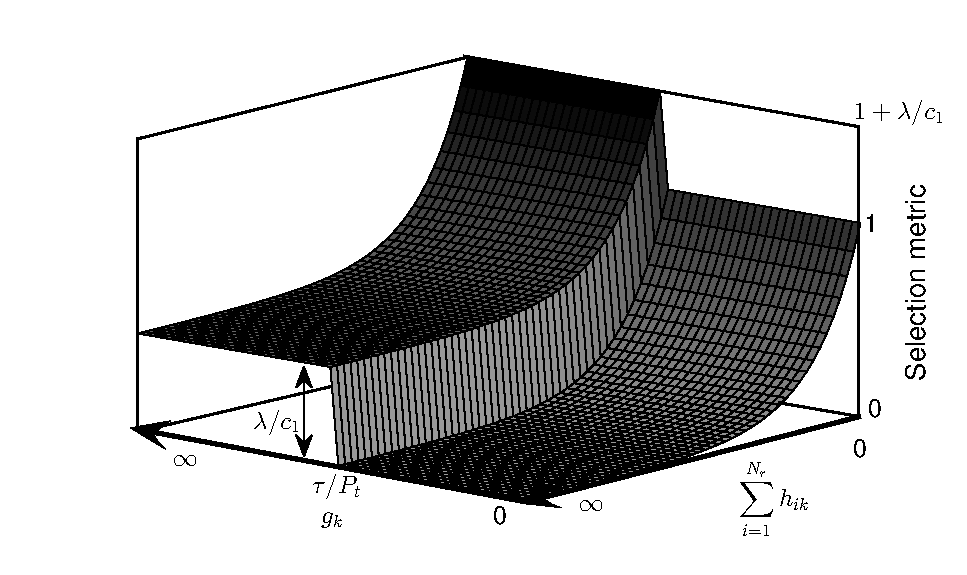
\includegraphics[width=\linewidth]{plots/selection_metric_3d.eps}
\caption{Selection metric of antenna $k$ as a function of $\sumnr\hk{ik}$ and $\gk{k}$.}
\label{fig:metric}
\end{figure}

\subsection{Interference-Outage Probability and Optimality of LWIIR}
We first derive the interference-outage probability of LWIIR in terms of the distribution of $\yk{1},\ldots,\yk{\Nt}$. Since $\yk{1},\ldots,\yk{\Nt}$ are identically distributed, we denote their marginal CCDF and PDF by $F_{y}^{c}(\cdot)$ and $f_{y}(\cdot)$, respectively. 
\begin{lemma}
\label{lem:outage_Nt}
The interference-outage probability $\outlam$ of LWIIR, for $0\leq\lam\leq\cone$, is given by
\begin{equation}
\label{eq:pr_outage_ccdf} 
\outlam  =  \Nt\un \int_{0}^{1-\lambym} 	
\left[ \un F_{y}^{c}\left(x\right) + \left(1 -\un\right)F_{y}^{c}\left(x+\lambym\right) \right]^{\Nt-1} f_{y}(x)\,dx.
\end{equation}
For the class of continuous fading models, $\outlam$ is a continuous and strictly monotonically decreasing function of $\lam$. Furthermore, for any $\outmax\in[0,\un]$, a unique $\lam\in[0,\cone]$ exists such that $\outlam=\outmax$. 
\end{lemma}
%
\begin{IEEEproof}
    The proof is given in Appendix~\ref{proof:outage_Nt}.
\end{IEEEproof}
%
%Note that~\eqref{eq:pr_outage_ccdf} reduces to $\un$ when $\lam=0$, which corresponds to the interference unconstrained rule. Further, $\outlam=0$ when $\lam=\cone$, which corresponds to the peak interference constrained rule.  

{\em Insights:} Replacing $x+\lambym$ with $\lambym$ in~\eqref{eq:pr_outage_ccdf}, the following closed-form upper bound for $\outlam$ can be derived: 
\begin{equation}
\label{eq:pr_outage_ub}
\outlam  \leq \left[ \un + \left(1-\un\right)F_{y}^{c}\left(\lambym\right)  \right]^{\Nt} - \left[ \un F_{y}^{c}\left(1-\lambym\right) + \left(1-\un\right)F_{y}^{c}\left(\lambym\right)  \right]^{\Nt}.
\end{equation}
For $\Nt = 2$, the following different, simpler bound can also be derived: 
\begin{equation}
\label{eq:two_Nt_UB}
\outlam \leq \un^2 + 2\un(1-\un)F_{y}^{c}\left(\lambym\right).
\end{equation}
For example for Rayleigh fading and $\Nr=1$ equating~\eqref{eq:two_Nt_UB} to $\outmax$ yields the following closed form upper bound for $\lam$, for $\itau\geq-\left( \Pt\mug/{2}\right) \ln\left({\outmax}\right)$:

\begin{equation}
\label{eq:two_Nt_lam}
\lam \leq \cone \left( \frac{2\un - \un^2 - \outmax}{2\un(1-\un)} \right)^{\snrbyal[]}.
\end{equation} 

Using Lemma~\ref{lem:outage_Nt}, we prove the following key result. 
%
\begin{theorem}
\label{thm:selection_rule_on_off}
The optimal TAS rule lies in the set of rules $\set{\callamrule:0\leq\lam\leq\cone}$. If $\outmax\geq\un$, then it is given by $\caluncons$. Else, for $0\leq\outmax<\un$, it is given by $\callamstarrule$, where $\lamstar>0$  is the solution of $\outlam=\outmax$. Such a choice of $\lamstar$ is unique, strictly positive, and always exists. 
\end{theorem}
%                
\begin{IEEEproof}
   The proof is given in Appendix~\ref{proof:selection_rule_on_off}.
\end{IEEEproof}
%

Notice that the optimal TAS rule only needs to know if the STx-PRx channel power gain exceeds a threshold $\tau/\Pt$. This makes it robust to errors in estimating $\g$. 

\section{SEP Analysis of LWIIR}
\label{sec:SEPanalysis}
 Having proved that LWIIR is SEP-optimal, we derive an expression for its average SEP, which we denote by  $\avgSEP$. We do this for the general case of $\Nt$ transmit antennas and $\Nr$ receive antennas for any continuous fading model. It turns out to be in a single integral form, which can be expressed as a summation using Gauss quadrature methods~\cite{abramowitz_stegun}. We gain insights by studying special cases for which the average SEP simplifies to a closed-form. %We conclude this section with asymptotic behavior of LWIIR as $\lam\tendsto\cone$. 
 
%In this section, we derive the average SEP expression for an interference-outage constrained underlay CR when LWIIR is employed. First, we do this for a secondary system with $\Nt$ transmit antennas and $\Nr$ receive antennas for any continuous fading model. Then, we show that this average SEP expression can be simplified to a closed-form for Rayleigh fading when $\Nr=1$.

\begin{theorem}
\label{thm:SEP_exact_Nt_gen}
$\avgSEP$ of $\callamrule$ for any continuous fading model is given by
\begin{equation}
\label{eq:SEP_Nt_gen} 
\avgSEP= m\left[\unccdfygen{\un}{1-\lambym}\right]^{\Nt} + \termtwo,
\end{equation}
%
where
\begin{align}
\label{eq:termtwo_gen}
\termtwo \!&= \Nt\m(1-\un)\int_{0}^{\lambym} \left[\un + \unccdfygen{(1-\un)}{x}\right]^{\Nt-1} x\pdfyNrgen{x} dx\nonumber\\
&\quad\quad\quad+ \Nt\m \int_{0}^{1-\lambym}
\left[\unccdfygen{\un}{x} +\unccdfygen{(1-\un)}{x+\lambym}  \right]^{\Nt-1}\nonumber\\
&\hspace{90pt}\times\left(\un x\pdfyNrgen{x} + (1-\un)\left(x + \lambym\right) \pdfyNrgen{x + \lambym}\right) dx.
\end{align}
%
\end{theorem}
%
\begin{IEEEproof}
The proof is given in Appendix~\ref{proof:SEP_exact_Nt_gen}.
\end{IEEEproof}
%

The first term in~\eqref{eq:SEP_Nt_gen} corresponds to the average SEP due to $s=\nx$. It increases as the interference-outage penalty factor $\lam$ increases. This is because a higher $\lam$ corresponds to a tighter interference-outage constraint, which increases the probability of selecting $s=\nx$. 
%
%\begin{multline}\label{eq:SEP_Nt_Nr_rayleigh} \frac{\Nt\m(1-\un)}{\Gamma(Nr)}\left(\albysnr\right)^{Nr}\int_{0}^{\lambym} \left(\un + \unccdfy{(1-\un)}{x}\right)^{\Nt-1} \ytimespdfyNr dx\\ + \frac{\Nt\m}{\Gamma(Nr)}\left(\albysnr\right)^{Nr} \int_{0}^{1-\lambym} \left(\unccdfy{(1-\un)}{\left(x+\lambym\right)} + \unccdfy{\un}{x}\right)^{\Nt-1}\\ \times\left((1-\un)\ypluslamtimespdfyNr+\un\ytimespdfyNr\right) dx\\ +m\left(\unccdfy{\un}{\left(1-\lambym\right)}\right)^{\Nt}.                                     \end{multline}

For Rayleigh fading, in which $\hk{ik}$ and $\gk{k}$ are i.i.d.\ exponential RVs with means $\muh$ and $\mug$, respectively, it can be shown that the unconstrained interference-outage probability $\un$ is equal to $\inlccdfg[]$. Thus, the optimal TAS rule is the same as the interference unconstrained rule $\caluncons$ $(\un\leq\outmax)$, for $\itau\geq\Pt\mug\ln\left(1/\outmax\right)$.  Let $\snr\define\Pt\muh/\noisevar$ denote the mean signal-to-noise-ratio (SNR) of the SU. Thus, the CCDF and PDF of the RV $\yk{1}$ are given by 
\begin{align}
\label{eq:ccdfyNr}
\ccdfyrv{x} &= \ccdfyNr{x}, \quad \text{for}\,\, x \in (0,1],\\
\label{eq:pdfyNr}
\pdfyNrgen{x} &= \pdfyNr, \quad \text{for}\,\,  x \in (0,1],
\end{align}
where $\gamma(\cdot,\cdot)$ denotes the lower incomplete gamma function~\cite[(8.350.1)]{gradshteyn00_book} and $\Gamma(\cdot)$ denotes the gamma function~\cite[(8.339.1)]{gradshteyn00_book}. Note that further simplification is not possible even for the special case due to the lower incomplete gamma function inside the integral.  
%
\subsection{Special Case: Rayleigh Fading and $\Nr=1$} 
For $\Nr=1$,~\eqref{eq:ccdfyNr} and~\eqref{eq:pdfyNr} simplify to $F_{y}^{c}(x) = 1-x^{\albysnr}$ and $f_{y}(x) = \al x^{\albysnr-1}/\snr$, for $x \in (0,1]$. Upon substituting these in~\eqref{eq:SEP_Nt_gen} and~\eqref{eq:termtwo_gen},  $\avgSEP$ simplifies to 
%
\begin{multline}
\label{eq:avgSEPoneNr} 
\avgSEP =\zerosep\un^{\Nt}\!\left[1-\left(1-\lambym\right)^{\!\albysnr[]}\right]^{\Nt}
+ \frac{\Nt\un^{\Nt}\al\lam}{\snr} \sum_{k=0}^{\Nt-1}\sum_{n=0}^{k} \frac{\nck{\Nt-1}{k} \nck{k}{n}\left(\lambym\right)^{\albysnr[(n+1)]}\left(1-\un\right)^{k+1} }{(-1)^{n} \left( \albysnr[(n+1)]+1\right)\un^{k+1} }\\ + \frac{\Nt\m\al}{\snr} \sum_{k=0}^{\Nt-1} \sum_{i=0}^{k} \sum_{j=0}^{\Nt-k-1} \binom{\Nt-1}{k} \binom{k}{i} \binom{\Nt-k-1}{j} \\\times(-1)^{i+j} \un^{k} (1-\un)^{\Nt-k-1} \left[ \un\psifun{j}{i+1} +  \left(1-\un\right) \psifun{j+1}{i} \right]
,
\end{multline}
where $\psifun{k_1}{k_2} = \int_{0}^{1-\frac{\lam}{\m}} \left(x+\lambym\right)^{\albysnr[k_1]} x^{\albysnr[k_2]} \,dx$.
%
In general $\psifun{k_1}{k_2}$ can be computed accurately as a sum of $n$  terms as follows: 
\begin{equation}
\psifun{k_1}{k_2} ={\onemlc^{\albysnr[k_2]+1}} \sum_{i=1}^{n} w_{i} {\left(\!x_i\onemlc +\lambym\right)}^{\albysnr[k_1]} x_i^{\albysnr[k_2]} + \text{o}\left(\frac{1}{n^2}\!\right),
\label{eq:gauss_quad}
\end{equation}
where $x_i$ and $w_i$ are the $n$ Gauss quadrature abscissas and weights~\cite{abramowitz_stegun}, respectively. In Section~\ref{sec:results}, we will see that this approximation is accurate even for $n$ as small as 4. Furthermore, for $\lam\in({\m}/{2}, \m]$, $\psifun{k_1}{k_2}$ can be written explicitly in terms of the following series~\cite{gradshteyn00_book}:
%
%\begin{multline}
%\psifun{k_1}{k_2} = \frac{\left(\lambym\right)^{\albysnr[k_1]} \left(1-\lambym\right)^{\albysnr[k_2]+1}}{\albysnr[k_2]+1} \\
%+ \sum_{\lidx=1}^{\infty}\! \frac{\akone\!\!\left(\akone\!-\!1\right)\!\ldots\!\left(\akone\!-\!\lidx\!+\!1\right)\!\left(\!\lambym\!\right)^{\!\!\albysnr[k_1]  - \lidx} \!\!\left(\!1\!-\!\lambym\!\right)^{\!\!\albysnr[k_2]+\lidx+1}}{\lidx ! \left(\albysnr[k_2]+\lidx+1\right)}. 
%\label{eq:inf_sum}
%\end{multline}

\begin{equation}
\psifun{k_1}{k_2} = \sum_{\lidx=0}^{\infty} \frac{\Gamma\left(\akone+1 \right) \left(\lambym\right)^{\albysnr[k_1]  - \lidx} \left(1-\lambym\right)^{\albysnr[k_2]+\lidx+1}}{\Gamma\left(\akone-\lidx+1 \right)\lidx ! \left(\albysnr[k_2]+\lidx+1\right)}. 
\label{eq:inf_sum}
\end{equation}
%
%Using Gauss quadrature~\cite{abramowitz_stegun}, 
%

%\subsection{Simpler TAS Rule and interference-outage Expressions}
\subsection{Insights: Simpler TAS Rule and Its Interference-Outage Probability}
In this section, we gain several insights about LWIIR when $\lam \tendsto \cone$. This happens when the probability that all the antennas are outage-incompatible exceeds $\outmax$, \ie, $\un^{\Nt}>\outmax$.    %$\prob{\gkgrtaubypt{1}}^{\Nt}>\outmax$.   
%

\newcommand{\gammath}{\gamma}
Let $\goodset$ denote the set of all outage-compatible antennas at a given time instant. First, consider the case when $\goodset$  is not empty. As $\lam \tendsto \cone$ from Comment 3 in Section~\ref{sec:lambda_rule} LWIIR becomes 
\begin{equation}
\label{eq:hp_rule}
s = \argmax_{k\in\goodset}\left\lbrace \sumnr \hk{ik}\right\rbrace. 
\end{equation}
Now, consider the case when $\goodset$ is empty. As all the antennas are outage-incompatible LWIIR becomes $s = \argmin\left\lbrace  \yk{0},\yk{1}+\lambym,\ldots,\yk{\Nt}+\lambym \right\rbrace$. Using $\yk{0}=1$,~\eqref{eq:yi_def}, and rearranging the terms we get
\begin{equation}
\label{eq:hp_rule}
s = \left\{
\begin{array}{ll}
0 , & \text{if}~\sumnr\hk{i1}\leq\gammath,\ldots, \sumnr\hk{i\Nt}\leq\gammath, \\
\argmax\limits_{k\in\antopts}\left\lbrace \sumnr\hk{ik}\right\rbrace , &\text{otherwise},
\end{array}\right.
\end{equation}
where $\gammath\define\igammainline$. Hence, a non-zero antenna is selected if and only if there is at least one antenna $k$ for which $\sumnr \hk{ik}$ exceeds the threshold $\gammath$ . Else, $s=0$. 


{\em Interference-Outage Probability} For the above TAS rule interference-outage happens only when $\goodset$ is empty and the STx  transmits with $s\neq\nx$. Hence,  $\outlam=\prob{{\goodset}=\nullset, s \neq 0}$. This can be shown to be equal to
\begin{equation}
\label{eq:pr_outage_hp}
 \outlam = \un^{\Nt} - \un^{\Nt}\left(\ccdfyrv{1-\lambym} \right)^{\Nt}.
 %\outlam  =  \un^{\Nt} - \un^{\Nt}\left[1 - \left(1-\lambym\right)^{\albysnr[]} \right]^{\Nt}.
\end{equation}
Alternatively,~\eqref{eq:pr_outage_hp} is the asymptotic expression for the interference-outage probability as $\lam\tendsto\cone$.

{\em Simpler Expression for $\lam$:} For Rayleigh fading and $\Nr=1$, equating~\eqref{eq:pr_outage_hp} with $\outmax$ yields the following closed-form expression for $\lam$ for $\itau<-\left({\Pt\mug}/{\Nt}\right) \ln\left({\outmax}\right)$: 
\begin{equation}
\label{eq:lam_asym}
 \lam  =  \cone - \cone\left(1 - \left[1 - \frac{\outmax}{\un^{\Nt}}\right]^{\frac{1}{\Nt}} \right)^{\snrbyal[]}.
\end{equation}
%
%This expression applies only when $\un^{\Nt}$ is greater than $\outmax$, which is equivalent to .  

%Note that the above upper bound will be less than or equal to $\cone$ only when $\frac{2\un - \un^2 - \outmax}{2\un(1-\un)}\leq 1$, which simplifies to $\un^2 \leq \outmax$, which is equivalent to $\itau\geq\left({\Pt\mug}/{2}\right)\ln\left(1/\outmax\right)$.
%which means for $\Pt<\frac{2\tau}{\mug\ln\left(1/\outmax\right)}$. 



\section{Impact of Imperfect CSI}
\label{sec:imperfectcsi}
We now study the behavior of LWIIR when the STx has imperfect estimates of the STx-SRx and STx-PRx channel power gains for Rayleigh fading as is invariably the case in practice. For tractability, we assume that the SRx knows the $\Nr$  complex channel gains corresponding to the transmit antenna selected perfectly. %We derive the analytical expressions for the interference-outage probability at the PRx and the average SEP of the SU with imperfect CSI. 


{\em Channel Estimation Model}: Let $\sugain{ik} = \sqrt{\hk{ik}}e^{-j\suchph_{ik}}\sim\CN\left(\muh\right) $ denote the complex baseband channel gain of the link from $\kth$ transmit antenna of the STx to the $\ith$ receive antenna of the SRx and $\pugain{k} = \sqrt{\gk{k}}e^{-j\puchph_{k}}\sim\CN\left(\mug\right)$ denote the complex baseband channel gain from the $\kth$ antenna of the STx to the PRx.  It can be shown that MMSE estimates of $\sugain{ik}$ and $\pugain{k}$, which are based on pilot transmissions by SRx and PRx with powers $\hpilotpower$ and $\gpilotpower$, respectively are  $\sugainhat{ik}\sim\CN\left(\muhhat \right)$ and $\pugainhat{k}\sim \CN\left(\mughat\right) $, where  $\muhhat ={\hpilotpower\mu^2_{\such}}/{\left( \hpilotpower\muh+1\right)}$ and $\mughat = {\gpilotpower\mu^2_{\puch}}/{\left( \gpilotpower\mug+1\right)}$~\cite{Kashyap_2014_TCOM}.  
This implies that the channel power gain estimates $\hkhat{ik}=|\sugainhat{ik}|^2$ and $\gkhat{k}=|\pugainhat{k}|^2$ are exponential RVs with means $\muhhat$ and $\mughat$, respectively. Furthermore, the correlation coefficient  of $\hk{ik}$ and $\hkhat{ik}$ is $\rhoh\define{\hpilotpower\muh}/{\left( \hpilotpower\muh + 1\right) }$, and that of $\gk{k}$ and $\gkhat{k}$ is $\rhog \define{\gpilotpower\mug}/{\left( \gpilotpower\mug + 1\right) }$. 


With imperfect CSI the antenna selected by LWIIR becomes 
\begin{equation}
\callamrule: s=\argmin\limits_{k\in\allopts} \left\{ \ykhatplusgkhat{k} \right\},
\label{eq:shat}
\end{equation}
%Recall that $\lamstar$ is obtained by equating interference-outage probability $\outlam$ with perfect CSI in~\eqref{eq:pr_outage_ccdf} to $\outmax$. 
where 
\begin{equation}
\ykhat{k} \define  \exp\left({- \frac{\Pt\sum_{i=1}^{\Nr}\hkhat{ik}}{\ctwo\noisevar} }\right), \quad \text{for} \quad 0\leq k \leq\Nt,
\label{eq:yihat_def}
\end{equation}
$\hkhat{1\nx} \define 0,\ldots,\hkhat{\Nr\nx} \define 0$, and $\gkhat{\nx}   \define 0$. Let $F_{\yhat}^{c}(\cdot)$ and $f_{\yhat}(\cdot)$ denote the CCDF and PDF of i.i.d. RVs $\ykhat{1},\dots,\ykhat{\Nt}$. Let the CCDF of i.i.d. RVs $\gkhat{1},\ldots,\gkhat{\Nt}$ be $\unhat\define\ccdfghatinline$ and  $\snrhat\define{\Pt\muhhat}/{\noisevar}$.  


\newcommand{\D}{D}
\newcommand{\pdfyhatNr}{\left(\ln\left(\frac{1}{x}\right)\right)^{\Nr-1}x^{\albysnr[]-1}} % only y terms constants taken care separately
\newcommand{\yhattimespdfyNr}{\left[-\ln\left(x\right)\right]^{\Nr-1}x^{\D}} % only y terms constants taken care separately
\newcommand{\yhatpluslamstartimespdfyNr}{\left[-\ln\left({x+\lamstarbym}\right)\right]^{\Nr-1}\left(x+\lamstarbym\right)^{\D}} % only y terms constants taken care separately
\newcommand{\yhatpluslamtimespdfyNr}{\left[-\ln\left({x+\lambym}\right)\right]^{\Nr-1}\left(x+\lambym\right)^{\D}} % only y terms constants taken care separately
\newcommand{\unccdfyhat}[2]{{#1}\,\,\ccdfyhatrv{#2}}


\newcommand{\avgSEPhat}{\widehat{\SEP}}

\subsubsection{ Average SEP} We now derive the average SEP expression of the above TAS rule in~\eqref{eq:shat}. %We do not give this for general fading model because ?? 

\begin{theorem}
\label{thm:avg_SEP_imperfect}
$\avgSEP$ of $\callamrule$ for an $\Nt\times\Nr$ CR system with imperfect CSI at the STx is given by
\begin{multline}
\label{eq:avg_SEP_imperfect}
\avgSEP = \frac{\Nt \T^{\Nr}\m(1-\unhat)}{\Gamma(\Nr)} \int_{0}^{\lambym} \left[\unhat + \unccdfyhat{(1-\unhat)}{x}\right]^{\Nt-1} \yhattimespdfyNr dx\\
\hspace{60pt} + \frac{\Nt \T^{\Nr}\m}{\Gamma(\Nr)} \int_{0}^{1-\lambym}
\left[\unccdfyhat{\unhat}{x} + \unccdfyhat{(1-\unhat)}{x+\lambym} \right]^{\Nt-1} \left(\unhat\yhattimespdfyNr \right. \\ 
\hspace{40pt}\left. + (1-\unhat)\yhatpluslamtimespdfyNr\right)\, dx 
+m\left[\unccdfyhat{\unhat}{1-\lambym}\right]^{\Nt}\!\!,\!\!
\end{multline}
where $F_{\yhat}^{c}\left(x\right) = \frac{\gamma\left(\Nr,-\albysnrhat[]\ln(x)\right)}{\Gamma(\Nr)}$, $\T \define \Tc$, and $\D \define \Dc$.	
\end{theorem}
\begin{IEEEproof}
	The proof is given in Appendix~\ref{proof:avg_SEP_imperfect_CSI}.
\end{IEEEproof}

%Substituting $\snrhat=\snr$, $\rhoh=1$, and $\unhat=\un$ in~\eqref{eq:avg_SEP_imperfect} reduces it to the average SEP expression for the perfect CSI case in~\eqref{eq:SEP_Nt_gen}. 
Further simplification of $\avgSEP$ in~\eqref{eq:avg_SEP_imperfect} is not possible. However, for $\Nr=1$ simplified expressions can be obtained similar to that of perfect CSI case in~\eqref{eq:avgSEPoneNr}. These are not shown here to conserve space.



\subsubsection{ Interference-Outage Probability} We now derive the interference-outage probability for the TAS rule in~\eqref{eq:shat}.

\begin{theorem}
\label{thm:outage_imperfect_CSI}
  The interference-outage probability $\outlam$ of $\callamrule$ with imperfect CSI is given by
\begin{multline}
\label{eq:pr_outage_impefect} 
\!\outlam \!=\! \Nt \!\int_{0}^{1-\lambym} 	
\!\left[ \unhat F_{\yhat}^{c}\left(x\right) + \left(1 -\unhat\right)F_{\yhat}^{c}\left(x+\lambym\right)\right]^{\Nt-1}\!\! \left(\! (\un - \Probglt) f_{\yhat}\left(x\right)  \!+\!  \Probglt f_{\yhat}\!\left(\! x+\lambym\right) \!\right) dx\\
+ \frac{ \Probglt}{1 - \unhat} \left( 1 - \left[\unhat + \left(1 -\unhat\right)F_{\yhat}^{c}\left(\lambym\right)  \right]^{\Nt}  \right) ,
\end{multline}
%
%\begin{multline}
%\label{eq:pr_outage_imperfect_ub}
%\outlam  \leq \frac{\un - \Probglt}{\unhat}\left( \left[\unhat + \left(1-\unhat\right)F_{\yhat}^{c}\left(\lambym\right)\right]^{\Nt} - \left[ \unhat F_{\yhat}^{c}\left(1-\lambym\right) + \left(1-\unhat\right)F_{\yhat}^{c}\left(\lambym\right)\right]^{\Nt}\right) \\+  \frac{ \Probglt \left( 1-\unhat^{\Nt}\right) }{1-\unhat},
%\end{multline}
%
%respectively,
where $\Probglt \!=\! \un  Q_1\!\left(\frac{\rhog}{ \gpilotpower} \sqrt{\frac{2\itau}{ \gpilotpower\Pt}},\sqrt{\frac{2 \gpilotpower\itau}{\Pt}}\right) \! - \frac{\unhat}{2} \left(\! 1 + e^{-\frac{2\itau\rhog}{ \gpilotpower\Pt}}I_{0}\!\left(\frac{2\itau\rhog}{ \gpilotpower\Pt} \right) \!\right)$, $I_{0}(\cdot)$ is the modified Bessel function of the zeroth order~\cite[(8.406.3)]{gradshteyn00_book}, and  $Q_1(\cdot,\cdot)$ is the Marcum-Q function~\cite[(4.34)]{simon_alouini_book}.  %,  and $f_{\yhat}\left( x\right) = \frac{ \left( \albysnrhat \right)^{\Nr} \left(-\ln\left(x \right)\right)^{\Nr-1} x^{\albysnrhat - 1}}{\Gamma(\Nr)}$.
\end{theorem}
%
\begin{IEEEproof}
	The proof is given in Appendix~\ref{proof:outage_imperfect_CSI}.
\end{IEEEproof}
%

Note: In the interference unconstrained case $\left(\lam=0\right)$, $\outlam$ in~\eqref{eq:pr_outage_impefect} reduces to $\un$ even for the imperfect CSI. This is because when $\lam=0$, the selected  antenna does not depend on the  STx-PRx channel power gain estimates. Furthermore, in the peak interference power constrained case $\left(\lam=\cone\right)$, it simplifies to $\frac{ \Probglt \left( 1-\unhat^{\Nt}\right) }{1-\unhat}$, which is zero for perfect CSI. Furthermore, we can derive a closed form upper bound similar to~\eqref{eq:pr_outage_ub} for~\eqref{eq:pr_outage_impefect} as well.





\section{Numerical Results and Performance Benchmarking}
\label{sec:results}
We now present Monte Carlo simulations that use $10^6$ data symbols to verify our analytical results  and study the behavior of LWIIR as a function of different system parameters. We also benchmark its performance against other TAS rules proposed in the literature and show the impact of imperfect CSI . We use  $\lam=\lamstar$, the optimal interference-outage penalty factor that equates $\outlam$ in~\eqref{eq:pr_outage_ccdf} to $\outmax$, for $\outmax < \un$ and $\lam=0$,  for $\outmax \geq \un$. We set $\noisevar =1$ and $\muh =\mug = 1$, and show for Rayleigh fading. 

%Figure~\ref{fig:SEP_vs_PT} plots the average SEP of  LWIIR as a function of the transmit power $\Pt$ for $\itau=8$~dB and $\Nr=2$. This is done for two values each of $\outmax$ and $\Nt$. We observe that the analysis expression in~\eqref{eq:SEP_Nt_gen} matches well with the simulations. To understand its behavior, the transmit power needs to be divided into three regions. Consider, for example, $\outmax=0.1$ and $\Nt=4$. (i) When $\Pt \leq 4.4$~dB: Here, the STx is in the {\em interference-outage unconstrained} region. Hence, LWIIR is same as the $\caluncons$, and its average SEP decreases as $\Pt$ increases. In general, this region is for $\Pt\leq{\tau}/{\left(\mug\ln\left(1/\outmax\right)\right)}$; it is independent of $\Nt$. (ii) When $4.4~\text{dB} <\Pt \leq 9~\text{dB}$: Here, the STx is in the {\em interference-outage constrained} region, in which $\lamstar$ is positive, but close to zero. Thus, the average SEP continues to decrease as $\Pt$ increase. (iii) When $\Pt > 9$~dB: Here, $\lamstar$ is large enough ($>0.02$)  that the probability of the event that the STx selects antenna zero is significant and increases as $\lamstar$ increases further. Its SEP, which is $1- ({1}/{M})$, dominates the average SEP. Thus, in this region the average SEP increases with $\Pt$. In practice, this increase can be eliminated by lowering the transmit power $\Pt$ to <in words ??> . For example it is $9$~dB for $\outmax=0.1$ and $\Nt=4$, and $\Pt$ to $6.7$~dB for $\outmax=0.1$ and $\Nt=2$. Notice that average SEP decreases as $\outmax$ increases, since the interference-outage constraint is relaxed. It also decreases significantly as $\Nt$ increases due to increased spatial diversity.      

%\begin{figure}
%  \centering \includegraphics[width=\linewidth]{plots/PCSI_gs_SEP_vs_Pt_pout_5_10_tau_8dB_Nt_4_2_Nr_2_M_4.eps}
%  \caption{Average SEP as a function of $\Pt$ for different values of $\outmax$ and transmit antennas ($\itau = 8$~dB, $\Nr=2$, and QPSK).}
%\label{fig:SEP_vs_PT}
%\end{figure}


Figure~\ref{fig:SEP_vs_tau} plots the average SEP of LWIIR as a function of the interference power threshold $\itau$ for different values of transmit antennas at the STx and receive antennas at the SRx. The average SEP expression in~\eqref{eq:SEP_Nt_gen} is shown. Also shown is the average SEP obtained by simulating the entire transmit and receive chains and not assuming the formula in~\eqref{eq:isep}. We observe that the analysis matches well with the simulations. To understand the average SEP behavior, the interference power threshold is divided into two regions. (i) $\itau < 8.6$~dB: Here, the STx is in {\em interference-outage constrained} ($\outmax < \un$) region and hence $\lam>0$. We see that the average SEP decreases as $\itau$ increases because the interference power allowed at the PRx increases. 
%Note that the rate of decrease increases with the number of antennas. 
In general, this region is for $\itau < \Pt\mug\ln\left(1/\outmax\right)$; it is independent of $\Nt$ and $\Nr$.
(ii) $\itau \geq 8.6$~dB: Here, the STx is in {\em interference-outage unconstrained} ($\outmax \geq \un$) region and hence $\lam=0$. The average SEP saturates to a constant value as the optimal TAS rule becomes same as the interference unconstrained rule $\caluncons$. This constant value decreases significantly with increase in the number of antennas due to increased spatial diversity.

\begin{figure}
  \centering 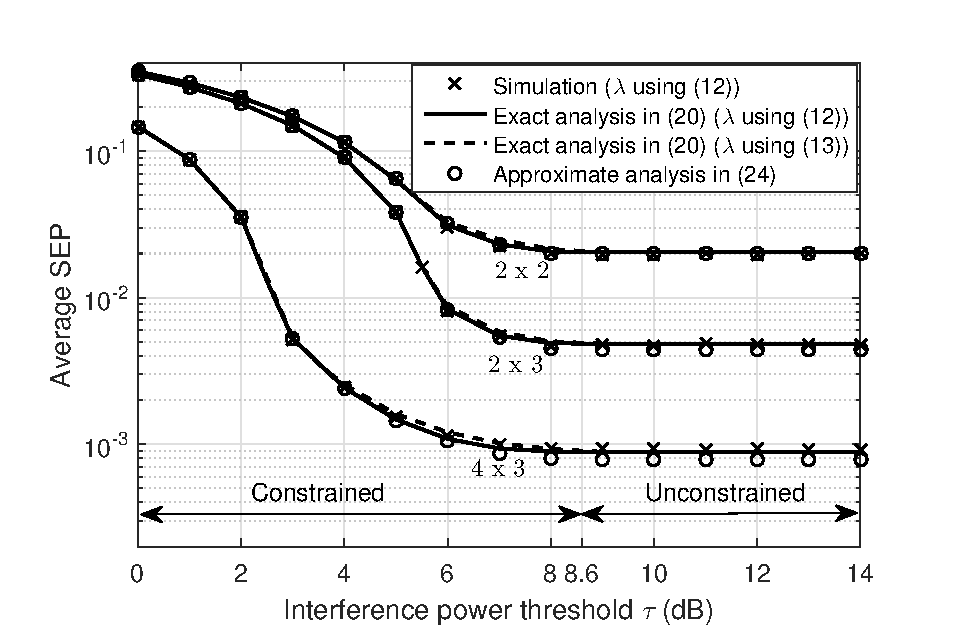
\includegraphics[width=\linewidth]{plots/PCSI_SEP_vs_tau_pout_10_PT_5dB_Nt_2_4_Nr_2_3_M_4.eps}
  \caption{Average SEP as a function of interference power threshold $\itau$ for different values of $\Nt$ and $\Nr$ ($\outmax=0.1$,  $\Pt = 5$~dB, and QPSK).}
\label{fig:SEP_vs_tau}
\end{figure}

Figure~\ref{fig:SEP_vs_tau_QAM} plots the average SEP as a function of the interference power threshold $\tau$. This is done for 8-PSK and 16-QAM, and for two values of $\outmax$. The simplified average SEP formula for $\Nr=1$ in~\eqref{eq:avgSEPoneNr} and its approximation in~\eqref{eq:gauss_quad} with $n = 4$ for 16-QAM and $n=8$ for 8-PSK  are shown. We observe that both~\eqref{eq:avgSEPoneNr} and~\eqref{eq:gauss_quad} match well with simulations. In the interference-outage constrained region the average SEP improves with increase in $\outmax$ as the maximum interference-outage allowed increases. In the interference-outage unconstrained region the average SEP floors to a constant value independent of $\outmax$.  %This boundary value is independent of the  constellations size and is equal to $16.6$~dB when $\outmax=0.1$. 

\begin{figure}
	\centering 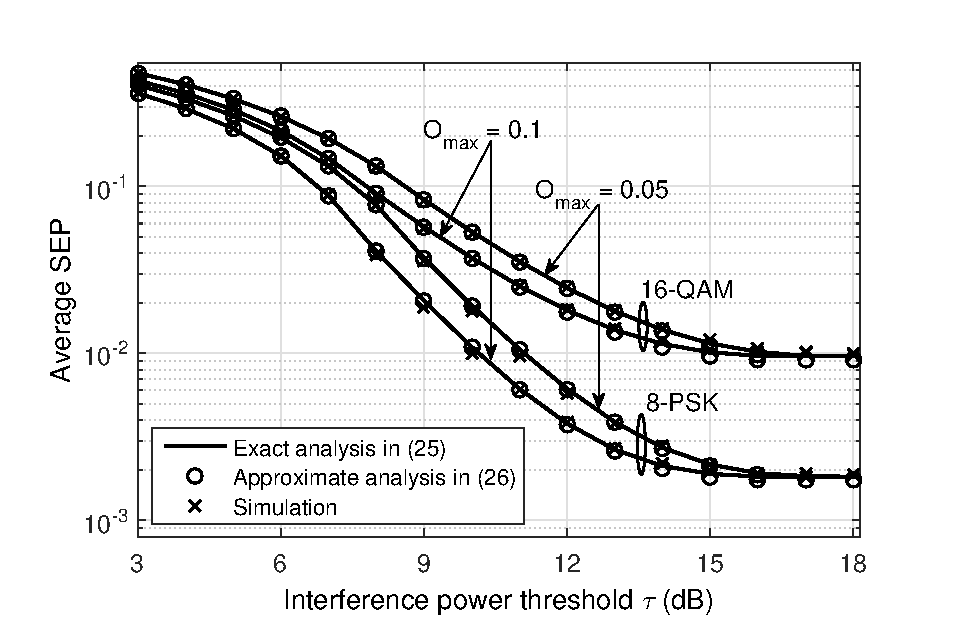
\includegraphics[width=\linewidth]{plots/CURVE_FIT_SEP_vs_tau_pout_5_10_PT_13dB_Nt_8_M_8_16.eps}
	\caption{Average SEP as a function of interference power threshold $\itau$ for 8-PSK and 16-QAM for different values of $\outmax$ ($\Pt = 13$~dB, $\Nt=8$, and $\Nr=1$).}
	\label{fig:SEP_vs_tau_QAM}
\end{figure}



%Figure~\ref{fig:outage_vs_lambym} plots the interference-outage probability as a function of the normalized interference-outage penalty factor $\lam/\cone$.  We see that the analytical expression in~\eqref{eq:pr_outage_ccdf} matches well with the simulations. Also plotted are the upper bounds in~\eqref{eq:pr_outage_ub} and~\eqref{eq:two_Nt_UB} and the asymptotic expression in~\eqref{eq:pr_outage_hp}. We observe that upper bound in~\eqref{eq:pr_outage_ub} becomes tighter as $\lam$ increases. Furthermore, the asymptotic expression in~\eqref{eq:pr_outage_hp} also matches with the exact  expression as $\lam$  tends to $\cone$.

%\begin{figure}
%  \centering \includegraphics[width=\linewidth]{plots/outage_vs_lambym_tau_10dB_PT_8dB_Nt_2_M_4.eps}
%  \caption{Interference-outage probability as a function of normalized interference-outage penalty factor $\lam/\m$ ($\itau = 10$~dB, $\Pt = 8$~dB, $\Nt = 2$, $\Nr=1$, and QPSK).}
%\label{fig:outage_vs_lambym}
%\end{figure}

{\em Performance Benchmarking:} We now compare the performance of the optimal TAS rule with the following rules:
\begin{itemize}
\item {\em Enhanced Minimum Interference (EMI) rule~\cite{Sarvendranath_2013_TCOM}}: Among the antennas $1,\ldots,\Nt$ it selects the one with the lowest STx-PRx channel power gain. However, it selects antenna $0$ when all the STx-PRx channel power gains are above a threshold, which is chosen to meet the interference constraint. 

\item {\em Enhanced Maximum-Signal-Power to Leak-Interference-Power-Ratio (EMSLIR) rule~\cite{Sarvendranath_2013_TCOM}}: Among the antennas $1,\ldots,\Nt$ it selects the one with the largest ratio of the STx-SRx channel power gain to the STx-PRx channel power gain. However, it selects antenna $0$ when these ratios of all the antennas are below a threshold, which is chosen to meet the interference constraint with equality. It is a relevant benchmark as it maximizes the SU capacity under the peak interference power constraint~\cite{Wang_2010_TWC}. 

\item {\em Difference Selection (DS) rule~\cite{Wang_2011_TCom,Sarvendranath_2014_TCOM}}: Among the antennas $1,\ldots,\Nt$ it selects the one that maximizes the difference $\delta \sumnr\hk{ik} -(1-\delta) \gk{k} $, where $\delta$ is chosen to meet the interference constraint with equality.   

\end{itemize}
Figure~\ref{fig:BM_SEP_vs_tau} compares the average SEPs of $\callamstarrule$, EMI, EMSLIR, and DS rules. The behavior again depends on the region in which $\callamstarrule$ operates. (i)~For $\itau < 15.6$~dB, it is in the interference-outage constrained region ($\lamstar>0$) and outperforms all the benchmark rules. For example, at $\itau=13$~dB,  its average SEP is lower by a factor of $79$, $12$, and $11$ than the EMI, EMSLIR, and DS rules. (ii)~For $\itau \geq 15.6$~dB, it is in the interference-outage unconstrained region. The average SEPs of $\callamstarrule$ and the DS rule saturate to same value. This is because the interference-outage constraint becomes inactive, and both rules reduce to the interference unconstrained rule $\caluncons$ in~\eqref{eq:uncons_simple}. While the average SEPs of EMI and EMSLIR also saturate, these values are 1-2 orders of magnitude larger. Also plotted is the average SEP of $\callamstarrule$ when $\lamstar$ is obtained by equating the integral-free interference-outage probability upper bound in~\eqref{eq:pr_outage_ub} to $\outmax$. We see that the degradation in the average SEP  is negligible when compared to using the exact $\lamstar$ from~\eqref{eq:pr_outage_ccdf}. 

\begin{figure}
	\centering 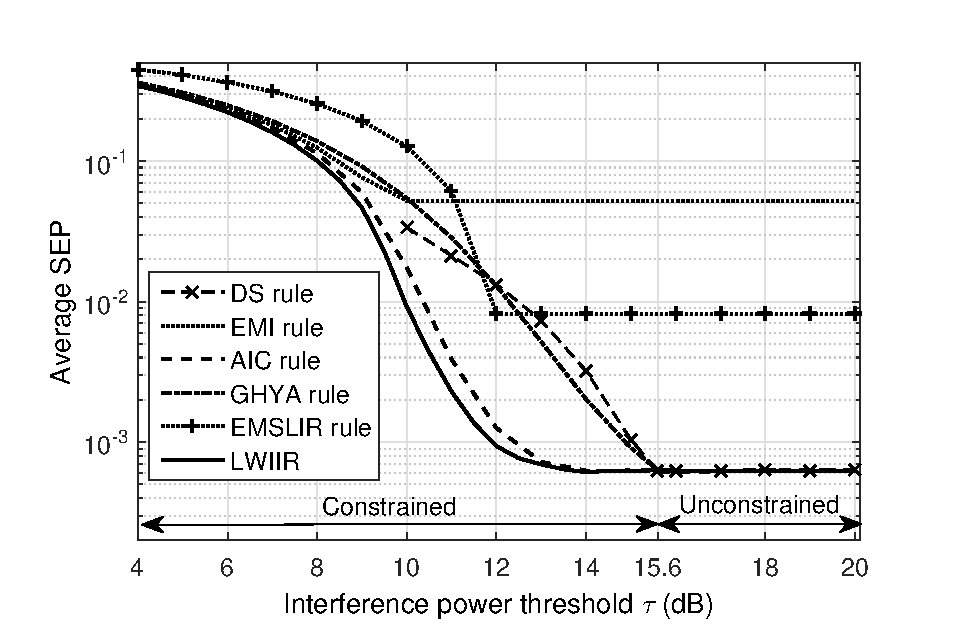
\includegraphics[width=\linewidth]{plots/BM_gs_SEP_vs_tau_pout_10_PT_12dB_Nt_4_M_4.eps}
	\caption{Performance benchmarking: Average SEPs of optimal TAS rule and several rules proposed in the literature ($\outmax = 0.1$, $\Pt = 12$~dB, $\Nt = 4$, $\Nr=1$, and QPSK).}
	\label{fig:BM_SEP_vs_tau}
\end{figure}


{\em Impact of Imperfect CSI:} Figures~\ref{fig:out_vs_tau_imp_CSI} and~\ref{fig:sep_vs_tau_imp_CSI} show the impact of imperfect CSI on the interference-outage and the average SEP of $\callamstarrule$ as a function of $\tau$. The imperfect $\Hmx$ ($\hpilotpower=5$~dB and $\gpilotpower=\infty$~dB) and imperfect $\g$ ($\hpilotpower=\infty$~dB and $\gpilotpower=5$~dB) cases are compared with the perfect CSI case. We observe that simulation results are in agreement with the analysis in all cases in both figures. The impact of imperfect CSI is different in the interference-outage constrained and interference-outage unconstrained regions. 

{\em Interference-Outage Constrained Region ($\itau\leq13.6$~dB):} Here, with perfect CSI the interference-outage probability is exactly $\outmax=0.1$. With imperfect $\g$, the interference-outage probability always exceeds  $\outmax$, because the probability of selecting an outage-incompatible antenna increases. This also results in a  lower average SEP compared to perfect CSI. The trends are different for the imperfect $\Hmx$. Here, the interference-outage probability is below $\outmax$, for $\itau\leq10.6$~dB, and above $\outmax$, for $\itau>10.6$~dB. Another difference is that the average SEP is always worse compared to perfect CSI.    

{\em Interference-Outage Unconstrained Region ($\itau>13.6$~dB):} Here, the interference unconstrained rule $\caluncons$ is optimal. The interference-outage probability becomes $\un$ for all the 3 cases, and it decreases exponentially as $\itau$ increases. Thus, in this region, imperfect CSI does not impact the interference-outage probability. We also see that the average SEP with imperfect $\g$ saturates to the same value as the perfect CSI. However, with imperfect $\Hmx$, it saturates to a higher value. %Thus, in this region the average SEP saturation value depends only on the quality of the STx-SRx channel.  

\begin{figure}
	\centering 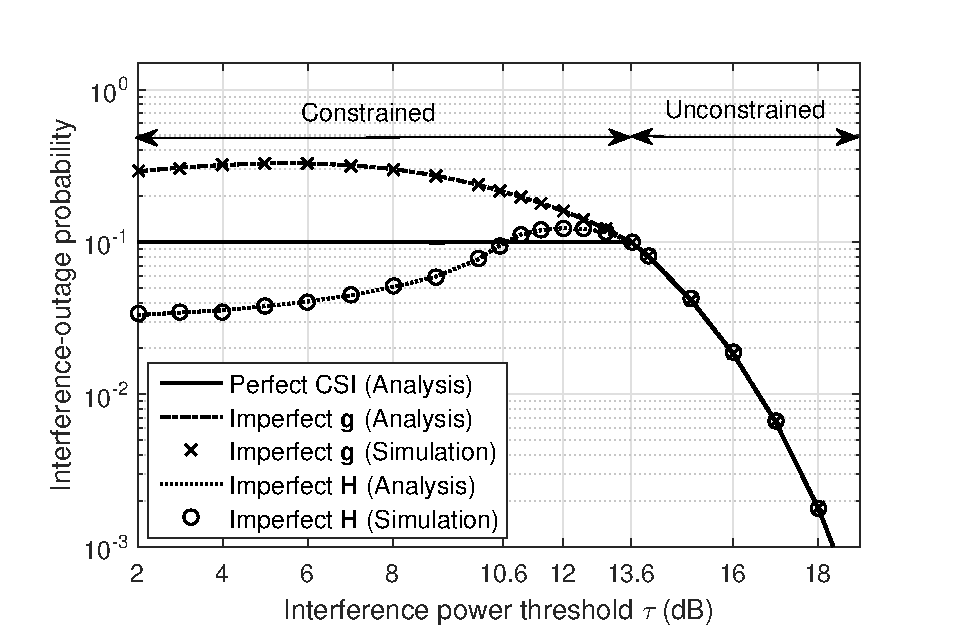
\includegraphics[width=\linewidth]{plots/Combined_outage_vs_tau_pout_10_PT_10dB_Nt_2_Nr_2_M_4.eps}
	\caption{Imperfect CSI: Interference-outage probability as a function of $\itau$ ($\outmax=0.1$, $\Pt = 10$~dB, $\Nt = 2$, $\Nr = 2$, and QPSK).}
	\label{fig:out_vs_tau_imp_CSI}
\end{figure}


\begin{figure}
	\centering 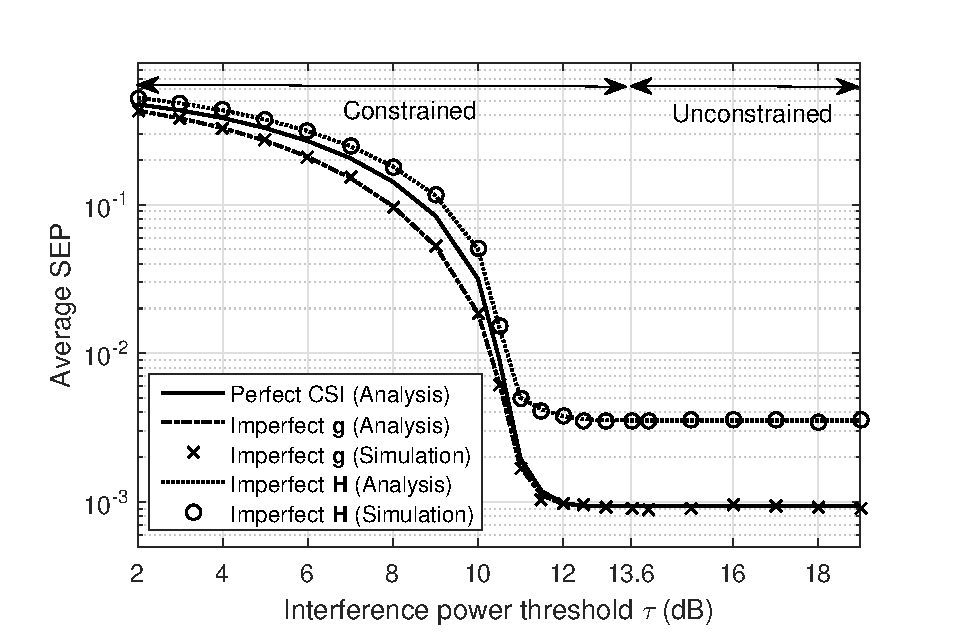
\includegraphics[width=\linewidth]{plots/Combined_SEP_vs_tau_pout_10_PT_10dB_Nt_2_Nr_2_M_4.eps}
	\caption{Imperfect CSI: Average SEP as a function of $\itau$ ($\outmax=0.1$, $\Pt = 10$~dB, $\Nt = 2$, $\Nr = 2$, and QPSK).}
	\label{fig:sep_vs_tau_imp_CSI}
\end{figure}




\section{Conclusions}
\label{sec:conclusions}
We proposed a novel and SEP-optimal TAS rule called LWIIR for an interference-outage constrained underlay CR. We showed that LWIIR was a discontinuous function of the STx-PRx channel power gain and is different from the naive approach in which a non-zero antenna is selected if its sum of STx-SRx channel power gains is above a threshold. However, it is optimal when all the antennas are outage-incompatible and lambda is very close to $\cone$. We also showed that LWIIR is applicable for a general class of fading models and for many constellations. We derived an exact average SEP expression for an SU with an arbitrary number of transmit and receive antennas. We further simplified it to an integral free closed-form expression for an SU with single antenna SRx and for Rayleigh fading. We showed that the proposed rule provides significant performance gain compared to other TAS rules in the literature. Extending this model to multiple PRxs and antenna subset selection would be an interesting problem for future work.

\appendix
\subsection{Proof of Lemma~\ref{lem:outage_Nt}}
\label{proof:outage_Nt}
We first derive the expression in~\eqref{eq:pr_outage_ccdf}. An interference-outage, i.e., $\Pt \gk{s} > \itau$, occurs only when $s\neq0$. Thus, using the law of total probability, the interference-outage probability $\outlam = \prob{\gkgrtaubypt{s}}$ is given by
%
\begin{equation}
\outlam =  \sum_{i=1}^{\Nt}\text{Pr}\brac{s=i,\gk{i}>\taubypt}=\Nt\text{Pr}\brac{s=1,\gk{1}>\taubypt}.
\label{eq:out_1}
\end{equation}
%
The second equality above follows due to symmetry.

Let $k$ antennas out of the antennas $2,\ldots,\Nt$ be outage-compatible. The total number of ways in which such $k$ antennas can be chosen from $\Nt-1$ antennas is $\nck{\Nt-1}{k}$. Given $k$, all these combinations are equally likely as the STx-PRx channels are i.i.d. One such combination in which antennas $2,\ldots,k$ are outage-compatible is $\setAk=\left\{\gklttaubypt{2},\dots,\gklttaubypt{k+1}, \gkgrtaubypt{k+2},\dots,\gkgrtaubypt{\Nt}\right\}$. Therefore, using the law of total probability, we can write $\outlam$ in~\eqref{eq:out_1} as
%
\begin{equation}
\outlam \!=\!\Nt\sum_{k=0}^{\Nt-1}\nck{\Nt-1}{k} \text{Pr}\brac{s = 1,\gk{1}>\taubypt,\setAk} \!=\!\Nt\sum_{k=0}^{\Nt-1}\nck{\Nt-1}{k}  \text{Pr}\brac{\setGk} \text{Pr}\brac{s = 1\Given \setGk},
\label{eq:out_3}
\end{equation}
%
where $\setGk\define\left\{\left(\gkgrtaubypt{1}\right)\cap\setAk \right\}$. Since $\gk{1},\ldots,\gk{\Nt}$ are i.i.d., we get $\prob{\setGk} = \left(1-\un\right)^k\un^{\Nt-k}$.
%

{\em Expression for $\prob{s = 1\Given\setGk}$:} Given $\setGk$, $\callamrule$ in~\eqref{eq:lam_weight_rule} selects antenna 1 if $\ykplambym{1}<\yk{i}$, for $2\leq i \leq k+1$,  $\ykplambym{1}<\ykplambym{j}$, for $k+2\leq j \leq \Nt$, and $\ykplambym{1}<\yk{0}=1$. Hence,
%
\begin{align}
\label{eq:out_5}
\!\!\!\prob{s = 1\Given \setGk }&\!=\!{\bf{E}}_{\yk{1}}\!\left[\prob{s = 1\Given\setGk,\yk{1}=x}\right] ,\\
\label{eq:out_51}
&\!=\!{\bf{E}}_{\yk{1}}\!\left[\text{Pr}\left(\xplambym < 1, \xplambym<\yk{2}, \dots ,\xplambym<\yk{k+1},\right.\right.\nonumber\\
&\quad\quad\quad\quad\quad\left.\left.
\xplambym<\ykplambym{k+2}, \dots ,\xplambym < \ykplambym{\Nt}\Given\setGk,\yk{1}=x\right)\right]\!.
\end{align} 
%

Conditioning on $\yk{1}$, the events in~\eqref{eq:out_51} are mutually independent. Furthermore, $\yk{2},\ldots,\yk{\Nt} $ are identically distributed. Hence, we get
%
%\begin{multline}
%\text{Pr}\brac{s=1\Given \setGk, \yk{1}=x} = \indic{x<1-\lambym}\left[\text{Pr}\brac{\yk{2}>x+\lambym\Given\yk{1}=x}\right]^{k}\\\times \left[\text{Pr}\brac{\yk{k+2}>x\given\yk{1}=x}\right]^{\Nt-k-1}.
%\label{eq:out_6}
%\end{multline}
\begin{equation}
\text{Pr}\brac{s=1\Given \setGk, \yk{1}=x} = \indic{x<1-\lambym}\left[\text{Pr}\brac{\yk{2}>x+\lambym}\right]^{k} \left[\text{Pr}\brac{\yk{k+2}>x}\right]^{\Nt-k-1}.
\label{eq:out_6}
\end{equation}
%
Substituting this in~\eqref{eq:out_5} and writing it in terms of the CCDF and the PDF of $\yk{1}$, we get 
\begin{equation}
\text{Pr}\brac{s=1\Given\setGk} =\int_{0}^{1-\lambym}\left[F_{y}^{c}\left(x+\lambym\right)\right]^k \left[F_{y}^{c}\left(x\right)\right]^{\Nt-k-1}f_{y}(x)\,dx.
\label{eq:out_7}
\end{equation}
Multiplying~\eqref{eq:out_7} with $\prob{\setGk}$ gives $\prob{s=1,\setGk}$. Substituting this in~\eqref{eq:out_3} and simplifying yields~\eqref{eq:pr_outage_ccdf}.

{\em Existence of $\lam$}: From~\eqref{eq:pr_outage_ccdf}: (i) We see that for the class of continuous fading models, $\outlam$ is an integral of a continuous and strictly decreasing  function in $\lam$. % Therefore, $\outlam$ is a continuous and strictly monotonically decreasing function of $\lam$. 
(ii) Furthermore, $\outlam=\un$ when $\lam=0$ and $\outlam=0$ when $\lam=\cone$. Thus, by the intermediate value theorem, for every $0\leq\outmax\leq\un$,  there exists a corresponding unique $\lam\in[0,\m]$ such that $\outlam=\outmax$. 
  

		

\subsection{Proof of Theorem~\ref{thm:selection_rule_on_off}}
\label{proof:selection_rule_on_off}
In order to prove that $\callamstarrule$ is optimal, we introduce the following terminology. First, we define a feasible selection rule to be a rule that satisfies the interference-outage constraint in~\eqref{eq:iop_cons}. Let $\F$ denote the set of all feasible rules. It is non-empty as the TAS rule that always selects antenna zero has an interference-outage probability of zero and is, therefore, feasible. Any TAS rule that violates~\eqref{eq:iop_cons} cannot be optimal. Thus, we can restrict our focus to the TAS rules in $\F$. We consider the two cases $\outmax\geq\un$ and $\outmax<\un$ separately below.

{\em 1. $\outmax\geq\un$:} From the discussion in Comment 1 in Section~\ref{sec:lambda_rule}, the interference unconstrained rule $\caluncons$ is feasible and is the optimal rule. 

{\em 2. $0\leq\outmax<\un$:} Here, the interference unconstrained rule is not feasible.  Instead, consider the TAS rule $\callamstarrule$, where $\lamstar$ is chosen such that the interference-outage probability of $\callamstarrule$ is equal to $\outmax$. From Lemma~\ref{lem:outage_Nt}, such a choice of $\lamstar$ always exists, is unique, and is strictly positive. For a given realization of $\yk{1},\ldots,\yk{\Nt}$, and $\gk{1},\ldots,\gk{\Nt}$, let $\sstar$ be the antenna selected by $\callamstarrule$. Then, among all the selection rules in $\F$, $\callamstarrule$, by its definition,  minimizes $\yk{{\sstar}} + \frac{\lamstar}{\cone}\gindic{{\sstar}}$. 

Consider any feasible rule $\asrule\in\F$, such that  $s=\phi(\Hmx,\g)$. From above, it follows that   
\begin{equation}
\label{eq:opt_rul_1}  
   \explow{\Hmx,\g}{\yk{{\sstar}} + \frac{\lamstar}{\cone}\gindic{{\sstar}}} \leq  \explow{\Hmx,\g}{\yk{{s}} + \frac{\lamstar}{\cone}\gindic{{s}}}.
\end{equation}
Substituting $\yk{i}={\SEP(\mathbf{\such}_{i})}/{\cone}$ (from~\eqref{eq:isep} and~\eqref{eq:yi_def}) and using $\explow{\Hmx,\g}{\gindic{i}}=\prob{\gk{i}>\taubypt}$, we get
%
\begin{equation}
\label{eq:opt_rul_2}
   \explow{\Hmx,\g}{\SEP(\hsstar)} + \lamstar  \prob{\gk{\sstar}>\taubypt} \leq  \explow{\Hmx,\g}{\SEP(\hs)} + \lamstar  \prob{\gk{s}>\taubypt}.
\end{equation}
%
We also know that $\prob{\gk{\sstar}>\taubypt}=\outmax$. By rearranging the terms, we get
%
\begin{equation}
\label{eq:ineq_3}
\explow{\Hmx,\g}{\SEP(\hsstar)} \leq \explow{\Hmx,\g}{\SEP(\hs)} + \lamstar \left( \prob{\gk{s}>\taubypt} -  \outmax \right).
\end{equation}
%
Since $\phi$ is a feasible rule, we know that $\prob{\gkgrtaubypt{s}}\leq \outmax$. As $\lamstar>0$,~\eqref{eq:ineq_3} implies that $\explow{\Hmx,\g}{\SEP(\hsstar)} \leq \explow{\Hmx,\g}{\SEP(\hs)}$ for any feasible rule $\phi$. %Thus, $\callamstarrule$ is optimal.




\subsection{Proof of Theorem~\ref{thm:SEP_exact_Nt_gen}}
\label{proof:SEP_exact_Nt_gen}
We start with the probability of error conditioned on $\y \define [\yk{1},\ldots,\yk{\Nt}]$  and $\g$, denoted by $\prob{\Err \given \y,\g}$. Using the law of total probability, it can be written as
%
\begin{equation}
\prob{\Err \given \y,\g} =  \prob{s=\nx,\Err\given\y,\g} + \sum_{i=1}^{\Nt}\prob{s=i,\Err\given\y,\g}.
\label{eq:Perr_all_h}
\end{equation}
%
Furthermore, $\prob{s=k,\Err\given\y,\g}=\prob{s=k\given\y,\g}\prob{\Err\given\y,\g,s=k}$, for $0\leq k \leq \Nt$. Averaging over $\y$ and $\g$ and exploiting symmetry, $\avgSEP$ is given by
\begin{multline*}
\label{eq:avg_SEP_1}
 \avgSEP = \explow{\y,\g}{\prob{s=\nx\given\y,\g}\prob{\Err\given\y,\g,s=\nx}} + \Nt\explow{\y,\g}{\prob{s=1\given\y,\g}\prob{\Err\given\y,\g,s=1}}. 
\end{multline*}

Given $s=0$, the SEP is equal to $\zerosep$.\footnote{Instead of $c_1$, we use the more accurate value of $\zerosep=1-\left( 1/M\right) $ for the SEP with zero transmit power.}  Thus, $\prob{\Err\given\y,\g,s=\nx}=\zerosep$. Given $s=1$, from~\eqref{eq:isep} and~\eqref{eq:yi_def}, we get $\prob{\Err\given\y,\g,s=1}=\m \yk{1}$. Hence,
\begin{equation}
\label{eq:avg_SEP_3}
\avgSEP  = \zerosep \explow{\y,\g}{\prob{s=\nx\given\y,\g}} + \Nt\m\explow{\y,\g}{\yk{1}\prob{s=1\given\y,\g}}.
\end{equation}
From the law of total expectation, we know that $\explow{\y,\g}{\prob{s=\nx\given\y,\g}} = \prob{s = 0}$.
Similarly, 
\begin{equation}
\label{eq:avg_sep_3_one}
\explow{\y,\g}{\yk{1}\prob{s = 1\given \y,\g} } = \explow{\yk{1}}{\yk{1} \prob{s = 1\given \yk{1}}  }.
\end{equation}

Substituting these  two results into~\eqref{eq:avg_SEP_3}, we get
%
%\begin{equation}
%\label{eq:avg_SEP_4}
$\avgSEP  = \termone + \termtwo$,
%\end{equation}
%
where $\termone=\zerosep \prob{s = 0}$ and $\termtwo=\Nt\m \explow{\yk{1}}{ \yk{1}\prob{s = 1\given \yk{1}}}$. We now evaluate $\termone$ and $\termtwo$.

{\em First Term $\termone$:}
From the selection rule in~\eqref{eq:lam_weight_rule}, we know that ${s=0}$ is selected when the selection metrics of antennas $1,\ldots,\Nt$ exceed $\yk{0}=1$, which happens only when they are outage-incompatible. Therefore, first term can be written as 
\begin{equation}
\termone = \zerosep\prob{\gkgrtaubypt{1},\dots,\gkgrtaubypt{\Nt}, \yk{1}\!+\!\lambym >1,\ldots,\yk{\Nt}\!+\!\lambym >1}.
\label{eq:termone_a}
\end{equation}
%
Using the fact that channels are i.i.d., and by writing the above formula in terms of the CCDFs of $\yk{1}$ and $\gk{1}$, we get the first term in~\eqref{eq:SEP_Nt_gen}.


{\em Second Term $\termtwo$}: From the law of total probability, we have 
%
\begin{equation}
\prob{s = 1\given \yk{1}} = \prob{s = 1,\gk{1}>\taubypt\Given\yk{1}}  + \prob{s = 1,\gk{1}\leq\taubypt\Given \yk{1}}. 
\label{eq:pr_s_1}
\end{equation}
%
Now, recall  the definition of the set $\setAk$ and the event  $\setGk=\left\{\left(\gkgrtaubypt{1}\right)\cap\setAk \right\}$ from Appendix~\ref{proof:outage_Nt}. Similarly, we define $\setLk\define\left\{\left(\gklttaubypt{1}\right)\cap\setAk \right\}$. Summing over all the events in which $k$ antennas out of the antennas $2,\ldots,\Nt$ are outage-compatible, we get in a manner similar to~\eqref{eq:out_3}:
\begin{multline}
\prob{s = 1\given \yk{1}} \! =\! \sum_{k=0}^{\Nt-1}\!\!\nck{\Nt-1}{k}\!\! 
\left[ \prob{s = 1 \Given \setGk , \yk{1}} \prob{\setGk} +  \prob{s = 1 \Given \setLk, \yk{1}} \prob{\setLk}\right].\!\! 
\label{eq:pr_s_1_2}
\end{multline}
% 
%Applying the chain rule, and using the fact that the STx-PRx channels are independent of $\yk{1}$, we get
%\begin{align} 
%\label{eq:prgrtaubypt}
%\prob{s = 1,\gkgrtaubypt{1},\setAk\Given \yk{1}} &= 
%\prob{s = 1\Given\gkgrtaubypt{1},\setAk, \yk{1}} \prob{\gkgrtaubypt{1},\setAk},\\  
%\prob{s = 1,\gklttaubypt{1},\setAk\Given \yk{1}} &= \prob{s = 1\Given \gklttaubypt{1},\setAk,\yk{1}}\prob{\gklttaubypt{1},\setAk}.
%\label{eq:prlttaubypt}
%\end{align}
%
The expression for $\prob{s = 1\given \setGk, \yk{1}}$ is given in~\eqref{eq:out_6}.  The expression for $\prob{s = 1\given \setLk, \yk{1}}$ can be derived along lines similar to that for $\prob{s = 1\given \setGk, \yk{1}}$ in~\eqref{eq:out_6}. This yields   
\begin{equation}
\text{Pr}\brac{s =1\given \setLk,\yk{1}=x} \!=\! F_{y}^{c}\brac{x}^{k}\left[\indic{x\leq\lambym} +\indic{x>\lambym}F_{y}^{c}\brac{x-\lambym}^{\Nt-k-1}\right].
\label{eq:prob_gklt}
\end{equation}
%
Substituting $\prob{\setGk}$ and~\eqref{eq:out_6} in~\eqref{eq:pr_s_1_2} simplifies the first part of~\eqref{eq:pr_s_1_2}. Similarly, using $\prob{\setLk}=\left(1-\un\right)^{k+1}\un^{\Nt-k-1}$ and~\eqref{eq:prob_gklt} simplifies the second part of~\eqref{eq:pr_s_1_2}. Substituting $\prob{s = 1\given \yk{1}}$ from~\eqref{eq:pr_s_1_2} in $\explow{\yk{1}}{ \yk{1}\prob{s = 1\given \yk{1}}}$ and averaging over $\yk{1}$ yields the final expression of $\termtwo$ in~\eqref{eq:termtwo_gen}. 


\subsection{Brief Proof of Theorem~\ref{thm:avg_SEP_imperfect}}
\label{proof:avg_SEP_imperfect_CSI}
The antenna $s$ selected by $\callamrule$  now depends on $\yhatvec\define\left[\ykhat{1},\ldots,\ykhat{\Nt} \right]$ and $\ghatvec\define\left[\gkhat{1},\ldots,\gkhat{\Nt} \right]$, while the SEP using the selected antenna $s$ is given by $\cone\yk{s}$.  Hence, to analyze the SEP, we now condition on $\y$, $\yhatvec$, and $\ghatvec$ as follows:
%
\begin{equation}
\prob{\Err \given \y,\yhatvec,\ghatvec} =  \prob{s=\nx,\Err\given \y, \yhatvec,\ghatvec} + \sum_{i=1}^{\Nt}\prob{s=i,\Err\given\y,\yhatvec,\ghatvec}.
\label{eq:Perr_all_imp_csi}
\end{equation}  
%
Averaging over $\y$, $\yhatvec$, and $\ghatvec$ and simplifying further in a manner similar to the steps from~\eqref{eq:Perr_all_h} to~\eqref{eq:avg_sep_3_one} in Appendix~\ref{proof:SEP_exact_Nt_gen}, we can show that
%
\begin{equation}
\label{eq:avg_SEP_3_IMP_CSI}
\avgSEP = \zerosep \prob{s=\nx} + \Nt\m\explow{\yk{1},\ykhat{1}}{\yk{1}\prob{s=1\given \ykhat{1}}}.
\end{equation}
%

The first term in~\eqref{eq:avg_SEP_3_IMP_CSI} can be obtained by replacing $\gk{i}$ with $\gkhat{i}$ and $\yk{i}$ with $\ykhat{i}$ in~\eqref{eq:termone_a}. The expectation in the second term can be written in terms of the joint PDF $f_{\yk{1}\ykhat{1}}\left(\cdot,\cdot\right)$ of the correlated RVs $\yk{1}$ and $\ykhat{1}$ as follows:
%
\begin{equation}
\label{eq:avg_SEP_4_IMP_CSI}
\explow{\yk{1},\ykhat{1}}{\yk{1}\prob{s=1\given \ykhat{1}}}= \int_{\xhat=0}^{1} \prob{s=1\given \ykhat{1}=\xhat} \left[ \int_{x=0}^{1} x  f_{\yk{1},\ykhat{1}}\left(x,\xhat\right)\,dx\right] \,d\xhat.
\end{equation}
%
We derive $\prob{s=1\given\ykhat{1}=\xhat}$ along lines similar to the steps from~\eqref{eq:pr_s_1} to~\eqref{eq:prob_gklt} in Appendix~\ref{proof:SEP_exact_Nt_gen},  by replacing $\yk{1}$ and $\gk{1}$ with $\ykhat{1}$ and $\gkhat{1}$. Thus, its final expression is obtained by replacing $\ccdfyrv{\cdot}$ and $\un$ with $\ccdfyhatrv{\cdot}$ and $\unhat$, respectively. 

{\em Joint PDF $f_{\yk{1},\ykhat{1}}\left(\cdot,\cdot\right)$:} First let us consider the joint PDF of two bivariate gamma RVs $V\define\sumnr\hk{i1}$ and $W\define\sumnr\hkhat{i1}$ which is given by~\cite[(6.1)]{simon_alouini_book}
\begin{multline}
\label{eq:bivargammaPDF}
f_{V,W}(v,w) = \frac{1}{\Gamma\left(\Nr \right) \left(1-\rhoh \right)\muh\muhhat }\left(\frac{vw}{\rhoh \muh\muhhat}\right)^{\frac{\Nr-1}{2}}\exp\left[{-\frac{1}{(1-\rhoh)}\left( \frac{v}{\muh}+\frac{w}{\muhhat}\right) } \right] \\ I_{\Nr-1}\left(\frac{2\sqrt{\rhoh vw}}{(1-\rhoh)\sqrt{\muh\muhhat}}\right),~\text{for}\; v,w>0,
\end{multline}
%  
where $I_{\Nr-1}\left(\cdot \right) $ is the modified Bessel function of $(\Nr-1)^{\text{th}}$ order. Now, we can obtain $f_{\yk{1},\ykhat{1}}\left(\cdot,\cdot\right)$ using the variable transformation $\yk{1}=\exp\left(-\Pt V/(\ctwo\noisevar) \right) $ and $\ykhat{1}=\exp\left(-\Pt W/(\ctwo\noisevar) \right)$ from~\eqref{eq:yi_def} and~\eqref{eq:yihat_def}, respectively, in~\eqref{eq:bivargammaPDF}.  
%
%\begin{multline}
%\label{eq:bivaratey1PDF}
%f_{\yk{1},\ykhat{1}}(x,\xhat) = \frac{1}{\Gamma\left(\Nr \right)\left(1-\rhoh \right)}\frac{\ctwo^{\Nr+1}}{\snr\snrhat} \left(\frac{\ln(x)\ln(\xhat)}{\rhoh \snr\snrhat}\right)^{\frac{\Nr-1}{2}} x^{\frac{\ctwo}{(1-\rhoh)\snr}-1 } \xhat^{\frac{\ctwo}{(1-\rhoh)\snrhat}-1 } \\ I_{\Nr-1}\left(\frac{2\ctwo}{(1-\rhoh)}\sqrt{\frac{\rhoh\ln(x)\ln(\xhat)}{ \snr\snrhat}}\right).
%\end{multline}
% 
Now, using $f_{\yk{1},\ykhat{1}}(\cdot,\cdot)$ we can  shown that $\int_{0}^{1} x f_{\yk{1}\ykhat{1}}\left(x,\xhat\right)\,dx = {T^{\Nr}\left(-\ln\left({\xhat} \right)\right)^{\Nr-1}\xhat^{D}}/{\Gamma\left(\Nr\right)}$.
%\begin{equation}
%\label{eq:y1_jpdf}
%\int_{x=0}^{1} x f_{\yk{1}\ykhat{1}}\left(x,\xhat\right)\,dx = \frac{T^{\Nr}\left(-\ln\left({\xhat} \right)\right)^{\Nr-1}\xhat^{D}}{\Gamma\left(\Nr\right)}.
%\end{equation}
Substituting this in~\eqref{eq:avg_SEP_4_IMP_CSI} and then in~\eqref{eq:avg_SEP_3_IMP_CSI}  yields~\eqref{eq:avg_SEP_imperfect}.



\subsection{Proof of Theorem~\ref{thm:outage_imperfect_CSI}}
\label{proof:outage_imperfect_CSI}
Instead of~\eqref{eq:out_1} we apply the law of total probability as follows for imperfect CSI:
\begin{equation}
\outlam=\Nt\text{Pr}\brac{s=1,\gk{1}>\taubypt,\gkhat{1}>\taubypt} + \Nt\text{Pr}\brac{s=1,\gk{1}>\taubypt,\gkhat{1}\leq\taubypt}.
\label{eq:outhat_2}
\end{equation}
Let $k$ be the number of STx antennas for which $\gkhatlttaubypt{i}$, for $2\leq i \leq\Nt$. Similar to $\setAk$, $\setLk$,  and  $\setGk$ in Appendices~\ref{proof:outage_Nt} and~\ref{proof:SEP_exact_Nt_gen}, we define $\setAkhat=\left\{\gkhatlttaubypt{2},\dots,\gkhatlttaubypt{k+1},\gkhatgrtaubypt{k+2},\dots,\gkhatgrtaubypt{\Nt}\right\}$, $\setLkhat\define\left\{\left(\gkhatlttaubypt{1}\right)\cap\setAkhat \right\}$, and $\setGkhat\define\left\{\left(\gkhatgrtaubypt{1}\right)\cap\setAkhat \right\}$. Then, along lines similar to~\eqref{eq:pr_s_1_2}, we can write~\eqref{eq:outhat_2}  as
%
\begin{multline}
\outlam =\Nt\sum_{k=0}^{\Nt-1}\nck{\Nt-1}{k}\left[ \prob{s = 1 \Given \gkgrtaubypt{1},\setLkhat} \prob{\gkgrtaubypt{1},\setLkhat} \right. \\  +\left.
\prob{s = 1 \Given\gkgrtaubypt{1}, \setGkhat } \prob{\gkgrtaubypt{1},\setGkhat}\right]   . 
\label{eq:pr_s_1_2_imp}
\end{multline}
%

First, let us consider the first term inside the summation in~\eqref{eq:pr_s_1_2_imp}:
\begin{enumerate}
\item  Given $\gkhatlttaubypt{1}$, from the definition of $s$ in~\eqref{eq:shat}, we know that the selection of antenna 1 does not depend on $\gk{1}$. Thus, $\prob{s = 1 \Given \gkgrtaubypt{1},\setLkhat}=\prob{s = 1 \given \setLkhat}$. This can be obtained by replacing $\ccdfyrv{\cdot}$ with $\ccdfyhatrv{\cdot}$ in~\eqref{eq:prob_gklt} and then averaging over $\yk{1}$. 

\item Using the fact that $\gkhat{2},\ldots\gkhat{\Nt}$ are independent of $\gk{1}$ and $\gkhat{1}$, we get  
\begin{equation}
\prob{\gkgrtaubypt{1},\setLkhat} =\prob{\gkgrtaubypt{1},\gkhatlttaubypt{1}}\prob{\setAkhat}. 
\end{equation}
Additionally, as $\gkhat{2},\ldots,\gkhat{\Nt}$ are i.i.d., we get $\prob{\setAkhat}=\left(1- \unhat \right)^{k} \unhat^{\Nt-k-1}$. We can also write
\begin{equation}
\label{eq:g1_integral}
\prob{\gkgrtaubypt{1},\gkhatlttaubypt{1}}=\int_{\xhat=0}^{\tau/\Pt}\int_{x=\tau/\Pt}^{\infty}f_{\gk{1},\gkhat{1}}\left(x,\xhat \right)\,dx d\xhat,
\end{equation}
where $f_{\gk{1},\gkhat{1}}\left(\cdot,\cdot \right)$ is the joint PDF of the bivariate exponential RVs $\gk{1}$ and $\gkhat{1}$.  This is a special case of~\eqref{eq:bivargammaPDF} with $\Nr=1$, and is obtained by replacing $\muh$, $\muhhat$, and $\rhoh$ with $\mug$, $\mughat$, and $\rhog$, respectively.
%\begin{equation}
\label{eq:bivargPDF}
%f_{\gk{1},\gkhat{1}}\left(x,\xhat \right) = \frac{\exp\left[{-\frac{1}{(1-\rhog)}\left( \frac{x}{\mug}+\frac{\xhat}{\mughat}\right) } \right]}{\left(1-\rhog \right)\mug\mughat}  I_{0}\left(\frac{2\sqrt{\rhog x\xhat}}{(1-\rhog)\sqrt{\mug\mughat}}\right),~\text{for}\; x,\xhat>0.
%\end{equation}
Then, evaluating the integral in~\eqref{eq:g1_integral} we get $\prob{\gkgrtaubypt{1},\gkhatlttaubypt{1}} \!=\! L$.
%\begin{equation}
%\prob{\gkgrtaubypt{1},\gkhatlttaubypt{1}} =  \un Q_1\left(\frac{\rhog}{ \gpilotpower} \sqrt{\frac{2\itau}{ \gpilotpower\Pt}},\sqrt{\frac{2 \gpilotpower\itau}{\Pt}}\right)  - \frac{\unhat}{2} \left( 1 + e^{-\frac{2\itau\rhog}{ \gpilotpower\Pt}}I_{0}\left(\frac{2\itau\rhog}{ \gpilotpower\Pt} \right) \right).
%\end{equation}

\end{enumerate}

Now, the second term inside the summation in~\eqref{eq:pr_s_1_2_imp}  can be simplified in a similar manner by repeating the above two steps.  Substituting these two results in~\eqref{eq:pr_s_1_2_imp} yields~\eqref{eq:pr_outage_impefect}.
 

\bibliographystyle{IEEEtran}
\bibliography{../../../Bibtex/bibJournalList,../../../Bibtex/standard,../../../Bibtex/sarvendra,../../../Bibtex/IEEE_papers,../../../Bibtex/mimo,../../../Bibtex/salil,../../../Bibtex/book}


%\bibliography{../../../Bibtex/sarvendra,../../../Bibtex/IEEE_papers}


\end{document}


